\documentclass[journal]{IEEEtran}
\IEEEoverridecommandlockouts

\usepackage{cite}
\usepackage{url}
\usepackage{amsmath,amssymb,amsfonts}
\usepackage{amsthm}
\usepackage{algorithmic}
\usepackage{graphicx}
\usepackage{textcomp}
\usepackage{xcolor}
\usepackage{booktabs}
\usepackage{multirow}
\usepackage{siunitx}
\usepackage{bm}
\usepackage{gensymb}
\usepackage{tikz}
\usetikzlibrary{arrows.meta, positioning, shapes.geometric, fit, backgrounds, calc, decorations.pathreplacing}

\def\BibTeX{{\rm B\kern-.05em{\sc i\kern-.025em b}\kern-.08em
    T\kern-.1667em\lower.7ex\hbox{E}\kern-.125emX}}

% Math shortcuts
\newcommand{\vR}{\mathbf{R}}
\newcommand{\vp}{\mathbf{p}}
\newcommand{\vv}{\mathbf{v}}
\newcommand{\va}{\mathbf{a}}
\newcommand{\vom}{\boldsymbol{\omega}}
\newcommand{\vg}{\mathbf{g}}
\newcommand{\vu}{\hat{\mathbf{u}}}
\newcommand{\vb}{\mathbf{b}}
\newcommand{\vz}{\mathbf{z}}
\newcommand{\vOm}{\boldsymbol{\Omega}}
\newcommand{\SO}{\mathrm{SO}(3)}
\newcommand{\so}{\mathfrak{so}(3)}
\newcommand{\Exp}{\mathrm{Exp}}
\newcommand{\Log}{\mathrm{Log}}
\newcommand{\calX}{\mathcal{X}}

% Review-markup macros from earlier drafts: now no-ops (the markup is kept in
% the sources where it still exists, so old diffs stay readable).
\newcommand{\rev}[1]{#1}
\newenvironment{revblock}{\par}{\par}

% --- Cut markup of the 2026-09-03 page review: items 2-7 were applied
%     (text deleted) on 2026-09-07, item 1 (fig:error_time) was kept.  The
%     macro stays defined for any future review pass.
\definecolor{cutred}{RGB}{185,0,0}
\newcommand{\cut}[2]{{\color{cutred}\textbf{[cut #1]} #2}}

% --- \anti{...}: an "X rather than Y" antithesis, flagged for review because
%     the construction reads as written-for-effect.  Keep it where the contrast
%     carries information, drop it where it is only rhetoric.  Each \anti stays
%     within one source line so the authorship colours cannot cut across it.
%     Grep for \anti{ to find them all; delete the wrapper to accept a phrase.
\newcommand{\anti}[1]{{\color{cutred}#1}}

% --- Cross-references: \autoref with IEEE-style names ---
\usepackage[hidelinks]{hyperref}
\renewcommand{\sectionautorefname}{Section}
\renewcommand{\subsectionautorefname}{Section}
\renewcommand{\subsubsectionautorefname}{Section}
\renewcommand{\figureautorefname}{Fig.}
\renewcommand{\tableautorefname}{Table}
\renewcommand{\equationautorefname}{Eq.}

% --- Acronyms: first \ac{} use writes out the long form + short; later
%     uses print the short form only (\printacronyms lists them). ---
\usepackage{acro}
\acsetup{list/template=tabular}  % auto-size the short-form column
% Acronym definitions (acro). Edit here; \ac{key} in the text.
\DeclareAcronym{rio}{short=RIO, long=radar-inertial odometry}
\DeclareAcronym{imu}{short=IMU, long=inertial measurement unit}
\DeclareAcronym{fmcw}{short=FMCW, long=frequency-modulated continuous-wave}
\DeclareAcronym{map}{short=MAP, long=maximum-a-posteriori}
\DeclareAcronym{rmse}{short=RMSE, long=root-mean-square error}
\DeclareAcronym{ransac}{short=RANSAC, long=random sample consensus}
\DeclareAcronym{nees}{short=NEES, long=normalized estimation error squared}
\DeclareAcronym{wls}{short=WLS, long=weighted least squares}
\DeclareAcronym{vio}{short=VIO, long=visual-inertial odometry}
\DeclareAcronym{slam}{short=SLAM, long=simultaneous localization and mapping}
\DeclareAcronym{ekf}{short=EKF, long=extended Kalman filter}
\DeclareAcronym{fej}{short=FEJ, long=first-estimates Jacobian}
\DeclareAcronym{ate}{short=ATE, long=absolute trajectory error}
\DeclareAcronym{rpe}{short=RPE, long=relative pose error}
\DeclareAcronym{snr}{short=SNR, long=signal-to-noise ratio}
\DeclareAcronym{mocap}{short=MoCap, long=motion capture}
\DeclareAcronym{lidar}{short=LiDAR, long=light detection and ranging}
\DeclareAcronym{uart}{short=UART, long=universal asynchronous receiver/transmitter}
\DeclareAcronym{com}{short=CoM, long=center of mass}
\DeclareAcronym{cad}{short=CAD, long=computer-aided design}


\begin{document}

\title{Continuous-Time Radar-Inertial Odometry\\with B-Spline Sliding-Window Optimization}

\author{Timo~Weiss%
\thanks{Guided Research project report (10 ECTS), Chair of Autonomous
Aerial Systems, Department of Aerospace and Geodesy, TUM School of
Engineering and Design, Technical University of Munich, Germany.
Supervisor: Lukas Pries.  Submitted Month~XX,~2026.}%
\thanks{Code and datasets are available at
\protect\url{https://github.com/Dr1zz3l/spline-rio}.}}

\maketitle

%------------------------------------------------------------------
\begin{abstract}
Millimeter-wave radar offers an alternative when visibility limits
optical sensing, but single-chip sensors provide sparse, noisy Doppler
returns.  This report investigates radar-inertial state estimation
during indoor quadrotor flight using a single-chip 60\,GHz radar
(TI IWR6843) and a 1\,kHz IMU, through flight regimes
from hover to aggressive racing and aerobatic backflips at
$10$\,rad/s.  We first characterize the radar
measurements against motion-capture ground truth.  A per-return
bearing-uncertainty law describes the Gaussian core, whose width grows
with transverse speed and off-boresight angle.  The errors also contain
a frame-shared component and outliers.  On the backflip flight, 38\% of
returns are Doppler-aliased.  The estimator uses a continuous-time
B-spline trajectory with one Doppler factor per return and a fixed-lag
smoother with marginalization.  A consensus front end rejects outliers,
while the per-return law, frame covariance, and measured stream error
budgets determine the weighting.  The measurement-derived noise model
and stream weights are held fixed across all evaluated flights and
platforms.
With reference yaw used as an idealized heading sensor, the causal
live-edge velocity RMSE is $0.16$--$0.28$\,m/s and orientation RMSE
is below $3\degree$ on racing, with position drift of
$0.3$--$1.3\%$ of path length.  Backflip velocity and orientation RMSE
rise to $1.66$\,m/s and $12.1\degree$, reflecting both radar measurement
limitations and the racing-oriented configuration.  The solver runs
in real time on a laptop CPU and reports conservative covariances on
the racing flights.  It transfers unchanged to a held-out fast-racing
flight, but performance degrades on a separate held-out flight with
extensive Doppler aliasing.  On four public flights from a
different platform with the same radar chip, velocity errors
are comparable to EKF baselines without retuning the noise model or
stream weights, although position drift is higher on three of the
four flights.  Radar and IMU with heading aiding thus provide a usable
velocity and orientation estimate; absolute position drifts with distance.
\end{abstract}

\begin{IEEEkeywords}
radar-inertial odometry, continuous-time estimation, B-spline,
sliding window, marginalization, mmWave radar, Doppler velocity
\end{IEEEkeywords}

% --- Declaration on the use of AI tools (required by the chair; DRAFT for
%     the author to adjust to the chair's wording) ---
\section*{Declaration on the Use of AI Tools}
Parts of the text of this report were formulated with the help of AI
language models (Anthropic Claude, OpenAI ChatGPT, Google Gemini)
from the author's notebooks,
measurements, worklog and instructions, and were subsequently revised
by the author throughout.  Model wording is most concentrated in
\autoref{sec:conclusion} (conclusion), \autoref{sec:results}
(results) and \autoref{sec:overview} (system overview), at $30$,
$28$ and $22$\,\% of their lines. The models were also used as a discussion
partner, for rewording and drafting text throughout, and for
software development support during the project.  All experiments and
measurements are the author's own, and the author takes full
responsibility for the entire content.

For transparency, a colour-coded copy of this report is published
alongside it as \texttt{report/main\_authorship.pdf} in the repository
above, with a key on each of its pages.  The marking is a
reconstruction from the commit history: the marked text is the model
wording that history can attribute.  Wording from earlier iterations
of the report predates the records that would identify a model, and
is left unmarked, as is wording introduced by any other means.
Only passages of at least three consecutive lines are marked, so the
copy shows blocks rather than scattered words.  It is an estimate of
origin, not a per-letter record of who typed what.

% ---- Body: one file per section (sections/) ----
\section{Introduction}
\label{sec:intro}

Visual odometry and \ac{lidar}-based \ac{slam} are well-established, but both
degrade in dusty, foggy, featureless, or textureless environments.
Millimeter-wave (mmWave) \ac{fmcw} radar is robust to these
conditions: it penetrates smoke and dust, operates in the dark, and
measures Doppler velocity directly without feature matching.  These
properties make it attractive for aggressive flight in unstructured
environments.

Combining a mmWave radar with an \ac{imu} (\ac{rio}) for ego-motion estimation
has been explored with discrete-time \ac{ekf} and graph-optimization
formulations~\cite{doer2020ekf,kramer2020rve}.  However,
asynchronous radar-\ac{imu} measurements (radar at $\sim$10\,Hz, \ac{imu} at
$\sim$1\,kHz) motivate a continuous-time trajectory, a smooth function
evaluated at any sensor timestamp without interpolation or preintegration.

\textbf{Research question.}
This work asks: \emph{can a single-chip mmWave radar,
fused with an \ac{imu} and a magnetometer, provide usable 6-DoF 
state estimation, and if so, what does it take?}  The starting point
is what the sensors can and cannot do: per-return Doppler yields
direct ego-velocity, but at around a dozen returns per frame there
aren't enough features for position fixing.
The system is therefore a \emph{velocity and orientation} source whose
position estimate drifts with distance.
\autoref{sec:char} characterizes the radar measurements.
The rest of the report develops an estimator informed by this
characterization and evaluates it from gentle to aerobatic flight.

We contribute:
\begin{itemize}
  \item a per-return characterization of a single-chip radar from
        hover to $10$\,rad/s, with every residual measured against
        motion capture ground truth: an uncertainty law with a
        per-return and a per-frame component, so one configuration is
        used for every evaluated flight and platform.
  \item a continuous-time \ac{rio} pipeline based on that characterization:
        every radar return is an individually weighted Doppler factor in a B-spline estimator, with a consensus front
        end, sensor-only initialization, and a fixed-lag smoother with
        a marginalization prior, running in real time on a laptop CPU.
  \item an evaluation from gentle racing to aerobatic backflips, on
        held-out flights and on a public cross-platform dataset
        against published \ac{ekf} baselines, including a consistency
        check of the reported covariance.
\end{itemize}

\textbf{Data and code.}
The complete system is released for independent reproduction.  The datasets
and our Ceres solver with Python bindings are available at
\url{https://github.com/Dr1zz3l/spline-rio}.

\section{Related Work}
\label{sec:related}

A survey~\cite{harlow2024survey} reviews mmWave radar in robotic
motion estimation, localization, and mapping.  We focus on
radar-inertial odometry for aerial platforms.

\textbf{Radar ego-velocity estimation.}
Doppler-based ego-velocity estimation from mmWave radar was
demonstrated by Kellner et al.~\cite{kellner2013instantaneous} and
extended to 3D with weighted least squares by
Kramer et al.~\cite{kramer2020rve}, whose RVE system fuses radar
with \ac{imu} in a discrete-time \ac{ekf}.  Doer and
Trommer~\cite{doer2020ekf} present an \ac{ekf}-based \ac{rio} with online
extrinsic calibration.  Our work uses per-frame \ac{wls}
ego-velocity estimates to initialize the position trajectory.
The continuous-time sliding-window optimizer uses one Doppler factor
per return (\autoref{sec:init}, \autoref{sec:robust}).

\textbf{Continuous-time trajectory estimation.}
Furgale et al.~\cite{furgale2013unified} introduced uniform B-splines
for continuous-time visual-inertial calibration.  The basalt
\ac{vio}~\cite{usenko2020basalt} uses cumulative B-splines on Lie groups
for stereo-inertial odometry; we adapt this basalt-style
cumulative SO(3) B-spline to radar-inertial fusion.

\textbf{Marginalization in sliding-window estimators.}
OKVIS~\cite{leutenegger2015keyframe} and
VINS-Mono~\cite{qin2018vins} use Schur complement
marginalization for visual-inertial systems, propagating information
from dropped keyframes as a dense Gaussian prior. We apply the same
principle to continuous-time B-spline control points.

\textbf{Continuous-time radar-inertial odometry.}
Ng et al.~\cite{ng2021ctrio} formulate continuous-time radar-inertial
odometry by fusing Doppler measurements from
\emph{multiple automotive} radars with an \ac{imu} as a least-squares
problem over a B-spline trajectory, evaluated on passenger vehicles.
Burnett et al.~\cite{burnett2025gp} use a Gaussian-process motion
prior for spinning-radar- and lidar-inertial odometry, and
\v{S}tironja et al.~\cite{stironja2026rio} model the \ac{imu} trajectory
continuously inside an \ac{rio} estimator with online spatio-temporal
calibration.  Yang et al.~\cite{yang2025gorio} (Go-RIO)
similarly fuse radar velocity with an \ac{imu} in continuous time and
target the same radar elevation drift with a ground-plane model, which
requires a persistently visible floor.  Our aerobatic flights see it
only intermittently.  Our front end rejects Doppler outliers but does
not impose a height constraint.  Huang et al.~\cite{huang2024lessismore}
exploit radar cross-section and Doppler physics to make a sparse
single-chip cloud usable in a discrete-time sliding-window
optimization, evaluated on ground-robot and handheld platforms.
We study a single-chip radar (10--60 points per frame,
12-channel array) on a quadrotor in aggressive racing and
\rev{aerobatic backflip} flight up to $10$\,rad/s.
The radar measurement errors increase in this regime
(\autoref{sec:backflips}).

\textbf{Single-chip \ac{rio} on aerial platforms.}
Single-chip radar-inertial fusion has also been evaluated on multirotors.
Michalczyk et al.~\cite{michalczyk2022ekf} use a
discrete-time \ac{ekf} with scan-to-scan point matching and Doppler (a
factor-graph reformulation follows in~\cite{michalczyk2024fg}); Girod et
al.~\cite{girod2024brio} run a real-time onboard M-estimator smoother on a
quadrotor in cities and forests, but cap velocity at
$2$\,m/s and anchor the vertical channel with a
barometer.  Our evaluation focuses on continuous-time estimation during
aggressive and \rev{aerobatic} flight, without a barometric height
measurement (\autoref{sec:baselines}).  None of the systems above
covers that combination.

\textbf{Sliding-window marginalization and consistency.}
Sliding-window marginalization can introduce inconsistency
in discrete time~\cite{dongsi2012consistency}, where \ac{fej}
methods fix linearization points to preserve the observability nullspace.
In continuous time, CLIC~\cite{lv2023clic} and
LIO-MARS~\cite{quenzel2025liomars} marginalize spline control points leaving the
window by adjacency to the dropped control points.  We follow the same
construction and account for the globally shared
\ac{imu} bias, which couples every \ac{imu} factor of the window and
requires care when selecting factors for marginalization
(\autoref{sec:sw}).

\textbf{Positioning against the \ac{ekf}-\ac{rio} baselines.}
In the discrete-time UAV line, the \ac{ekf}-\ac{rio} family of Doer and
Trommer~\cite{doer2020ekf} provides our comparison baselines.  Absolute
\ac{rmse} is not comparable across papers (firmware configuration alone
changes the Doppler resolution by an order of magnitude), so we
compare the systems on shared data:
\autoref{sec:baselines} runs our system on their public ICINS-2021
flights~\cite{doer2021yrio} and re-evaluates their estimators under
our causal metrics on the same data.

\section{Preliminaries}
\label{sec:prelim}

This section introduces the two mathematical tools the rest of the
report builds on: uniform B-splines as a continuous-time trajectory
representation, both in $\mathbb{R}^3$ and, in cumulative form, on
$\SO$; and the \ac{map} estimator that fits them to the measurements as
a weighted nonlinear least-squares problem. 

\subsection{Uniform B-splines in $\mathbb{R}^3$}
\label{sec:prelim_bspline}
An order-$N$ (degree $N{-}1$) uniform B-spline with control points
$\{\mathbf{P}_i\}\subset\mathbb{R}^3$ and constant knot spacing $\Delta t$
represents a curve as a weighted sum of basis functions,
\begin{equation}
  \vp(t) = \sum_i \mathbf{P}_i\, B_{i,N}(t),
  \label{eq:bspline_def}
\end{equation}
where the $B_{i,N}$ are the Cox--de Boor basis
functions~\cite{furgale2013unified}.  Two properties make this
representation attractive for asynchronous sensor fusion.

\emph{Local support.}  At any instant only $N$ consecutive control
points have nonzero basis, so on the segment $t\in[t_i,t_{i+1})$, with
normalized time $u=(t-t_i)/\Delta t\in[0,1)$, the curve is a fixed
blending of $N$ control points,
\begin{equation}
  \begin{gathered}
  \vp(t) = \sum_{j=0}^{N-1} B_j(u)\,\mathbf{P}_{i+j}, \\
  \bigl[B_0(u)\,\cdots\,B_{N-1}(u)\bigr]
     = \mathbf{u}^{\top}\mathbf{M}^{(N)},
  \end{gathered}
  \label{eq:bspline_blend}
\end{equation}
with $\mathbf{u}=[1,u,\dots,u^{N-1}]^{\top}$ and a constant $N\times N$
blending matrix $\mathbf{M}^{(N)}$~\cite{usenko2020basalt}.  Local
support limits each measurement's Jacobian to $N$ control points and
supports the marginalization described in \autoref{sec:sw}.

\emph{Analytic derivatives.}  Differentiating the basis in
\eqref{eq:bspline_blend} yields the velocity $\dot{\vp}(t)$ and
acceleration $\ddot{\vp}(t)$ in closed form at \emph{any} $t$, as
lower-order splines over the same control points, with no finite
differencing or inter-sample interpolation.  This is what lets the
accelerometer factor (which needs $\ddot{\vp}$) and the min-snap
regularizer (which needs $\vp^{(4)}$) be evaluated exactly at each
measurement's timestamp.  We use a quintic ($N{=}6$) position spline so
that snap is well defined and continuous.

\subsection{Cumulative $\SO$ B-splines}
\label{sec:prelim_so3}
Orientation lives on the manifold $\SO$, on which a weighted sum of
rotations $\sum_i \vR_i B_i$ is not itself a rotation, so
\eqref{eq:bspline_def} does not transfer directly.  The
\emph{cumulative} parameterization of Sommer et
al.~\cite{sommer2020efficient}, used in the basalt
\ac{vio}~\cite{usenko2020basalt}, instead writes the orientation as a
base rotation followed by a product of incremental rotations, each
mapped back onto the manifold by the exponential map,
\begin{equation}
  \begin{aligned}
  \vR(t) &= \vR_{i}
           \prod_{j=1}^{N-1}
           \Exp\!\bigl(\tilde{B}_j(u)\,\vOm_j\bigr), \\
  \vOm_j &= \Log\!\bigl(\vR_{i+j-1}^{-1}\vR_{i+j}\bigr)\in\so,
  \end{aligned}
  \label{eq:prelim_so3}
\end{equation}
where the increments $\vOm_j$ are the relative rotations between
consecutive \emph{absolute} orientation control points $\vR_i\in\SO$
(the optimization variables, basalt convention).  These orientation
control points are also called ``knots'' in the continuous-time
estimation literature~\cite{sommer2020efficient}; here, we use
``control points'' for both coefficient sets and reserve ``knots''
for the time values defining the spline intervals.  The cumulative
basis is the tail sum of the ordinary basis of \eqref{eq:bspline_blend},
\begin{equation}
  \tilde{B}_j(u) = \sum_{l=j}^{N-1} B_l(u).
  \label{eq:cumbasis}
\end{equation}
Because each $\Exp(\cdot)$ returns a rotation, $\vR(t)\in\SO$ holds by
construction for any orientation control points.  This form retains
absolute orientation control points, preserves local support over $N$
control points exactly as in the $\mathbb{R}^3$ case, and yields the body
angular velocity $\vom_b(t)$ in
closed form by differentiating the product, with no numerical
differentiation.  We use a cubic ($N{=}4$) orientation spline;
\eqref{eq:ori_spline} in \autoref{sec:state} is this construction with
$N{=}4$ (base control point $\vR_{k-3}$, three increments).

\subsection{\ac{map} Estimation as Weighted Least Squares}
\label{sec:prelim_map}
The control points and biases above form the finite-dimensional state
$\calX$ (\autoref{sec:problem}).  Each measurement $\vz_i$ relates to
the state through a known model $\mathbf{h}_i$,
$\vz_i = \mathbf{h}_i(\calX) + \mathbf{n}_i$, with the noise
$\mathbf{n}_i$ zero-mean Gaussian of covariance
$\boldsymbol{\Sigma}_i$ and independent across measurements.  The
likelihood is then
$p(\vz\mid\calX)\propto\prod_i
 \exp(-\tfrac12\mathbf{r}_i^{\top}\boldsymbol{\Sigma}_i^{-1}\mathbf{r}_i)$
with residuals $\mathbf{r}_i=\vz_i-\mathbf{h}_i(\calX)$, so its negative
logarithm is a weighted sum of squared residuals: maximum-likelihood
estimation minimizes
$\tfrac12\sum_i\mathbf{r}_i^{\top}\boldsymbol{\Sigma}_i^{-1}\mathbf{r}_i$,
in which each residual is weighted by its inverse covariance
(information) $\boldsymbol{\Sigma}_i^{-1}$.  For a scalar residual this
is a scalar weight $\lambda_i=1/\sigma_i^2$: a more certain sensor is
trusted more.  The variance measurements in \autoref{sec:char}
inform the stream weights $\lambda_a,\lambda_g$ of
\autoref{sec:models} and the per-return radar weights of
\autoref{sec:robust}.

Prior knowledge $p(\calX)$, here trajectory smoothness and, online, the
marginalization prior summarizing past data, turns the estimate into a
\ac{map} one, $\arg\max_{\calX} p(\vz\mid\calX)\,p(\calX)$; its negative
log contributes the extra quadratic terms $E_{\text{reg}}$ and
$E_{\text{prior}}$.  In a sliding window the prior is itself a
posterior: the previous window's posterior over the states both
windows share, with the states that left the window integrated out
(\autoref{sec:sw}).  Radar Doppler residuals have heavy tails
(\autoref{sec:char_noise} measures both the Gaussian core and the
tails); the identifiable outliers are removed before the solve
(\autoref{sec:char_outliers}), so every residual that reaches the
cost enters it quadratically.  Collecting all terms gives the weighted nonlinear
least-squares objective instantiated for our sensors in
\eqref{eq:map}.  We minimize it with Levenberg--Marquardt and
analytic Jacobians.  Rotation updates are applied on the manifold,
$\vR\mapsto\vR\,\Exp(\boldsymbol{\delta})$, so every iterate
remains a valid rotation.  The Jacobians use spline values and
derivatives at each measurement's exact timestamp, provided in
closed form by \autoref{sec:prelim_bspline} and
\autoref{sec:prelim_so3}.

\section{System Overview}
\label{sec:overview}

\subsection{Problem Formulation}
\label{sec:problem}

\textbf{Estimation problem.}
We estimate the continuous-time 6-DoF body trajectory (world-frame
position $\vp_w(t)\in\mathbb{R}^3$ and orientation $\vR(t)\in\SO$)
together with the constant \ac{imu} biases $\vb_a,\vb_g$, from asynchronous
measurements over \rev{a sliding estimation window}: radar Doppler velocities ($\sim$11\,Hz),
accelerometer and gyroscope samples (1\,kHz), and a low-rate heading
prior.  We adopt a \emph{continuous-time} representation because the
sensors are asynchronous and run at disparate rates: a trajectory defined
for every $t$ is evaluated at each measurement's exact timestamp, and its
derivatives (velocity $\dot{\vp}_w$, acceleration $\ddot{\vp}_w$, and
body angular velocity $\vom_b$) follow in closed form, so no
inter-sample interpolation or rigid-keyframe approximation is required.

\textbf{Parameterization.}
The position and orientation spline control points
(\autoref{sec:state}) and the \ac{imu} biases form the estimated state
\begin{equation}
  \mathcal{X} = \bigl\{\,\mathbf{P}_i,\ \vR_i,\ \vb_a,\ \vb_g\,\bigr\}.
  \label{eq:state}
\end{equation}
The radar extrinsics are fixed at their measured values.

\begin{figure}[t]
\centering
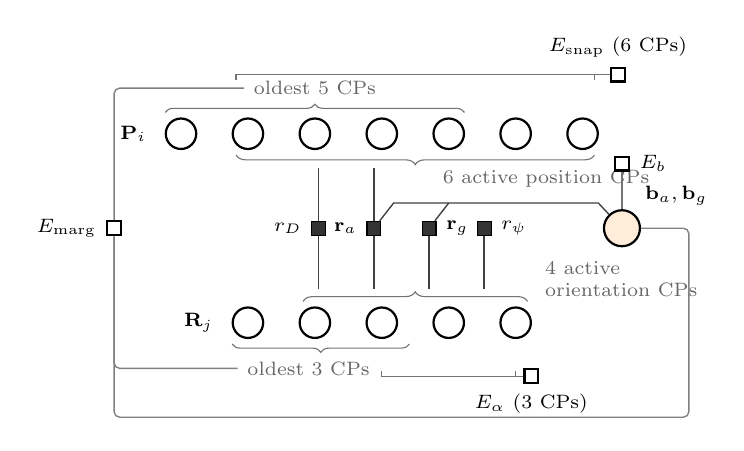
\begin{tikzpicture}[
  font=\footnotesize,
  var/.style={circle, draw, thick, fill=white, minimum size=11pt, inner sep=0pt},
  biasn/.style={circle, draw, thick, fill=orange!15, minimum size=13pt, inner sep=0pt},
  fac/.style={rectangle, draw, fill=black!80, minimum size=5pt, inner sep=0pt},
  reg/.style={rectangle, draw, thick, fill=white, minimum size=5pt, inner sep=0pt},
  edge/.style={black!75, line width=0.5pt},
  pedge/.style={black!50, line width=0.5pt, rounded corners=2pt},
  supp/.style={black!55, line width=0.5pt},
  lbl/.style={font=\scriptsize},
]
% rows: 7 position CPs, 5 orientation CPs
\foreach \i in {0,...,6}{ \node[var] (P\i) at (\i*0.85, 2.6) {}; }
\node[lbl, anchor=east] at (-0.32, 2.6) {$\mathbf{P}_i$};
\foreach \i in {0,...,4}{ \node[var] (R\i) at (0.85+\i*0.85, 0.2) {}; }
\node[lbl, anchor=east] at (0.53, 0.2) {$\vR_j$};
% active supports of the measurement factors (inner side of each row)
\draw[decorate, decoration={brace, mirror, amplitude=3.5pt}, black!55] (0.70, 2.33) -- (5.25, 2.33);
\draw[decorate, decoration={brace, amplitude=3.5pt}, black!55] (1.55, 0.47) -- (4.40, 0.47);
\node[lbl, black!60, anchor=west] at (3.2, 2.03) {6 active position CPs};
\node[lbl, black!60, anchor=west, align=left] at (4.50, 0.75) {4 active\\orientation CPs};
% measurement factors (inside both active spans)
\node[fac, label={[lbl]left:$r_{D}$}]            (fD)   at (1.75, 1.4) {};
\node[fac, label={[lbl]left:$\mathbf{r}_{a}$}]   (fa)   at (2.45, 1.4) {};
\node[fac, label={[lbl]right:$\mathbf{r}_{g}$}]  (fg)   at (3.15, 1.4) {};
\node[fac, label={[lbl]right:$r_{\psi}$}]        (fpsi) at (3.85, 1.4) {};
\draw[edge] (fD)   -- (1.75, 2.17);  \draw[edge] (fD)   -- (1.75, 0.63);
\draw[edge] (fa)   -- (2.45, 2.17);  \draw[edge] (fa)   -- (2.45, 0.63);
\draw[edge] (fg)   -- (3.15, 0.63);
\draw[edge] (fpsi) -- (3.85, 0.63);
% shared bias, right of the factor row: both IMU factors leave upward onto a
% common rail that clears the heading factor and its label
\node[biasn, label={[lbl]above right=-2pt and 0pt:$\vb_a,\vb_g$}] (b) at (5.6, 1.4) {};
\draw[edge] (fa) -- (2.70, 1.72) -- (5.30, 1.72) -- (b);
\draw[edge] (fg) -- (3.40, 1.72);
% outer side of the top row: prior (oldest 5 CPs) and min-snap (6 consecutive CPs)
\draw[decorate, decoration={brace, amplitude=3pt}, black!55] (-0.2, 2.87) -- (3.6, 2.87);
\node[lbl, black!60, anchor=south] (oldcp) at (1.7, 2.97) {oldest 5 CPs};
\draw[supp] (0.70, 3.28) -- (0.70, 3.35) -- (5.25, 3.35) -- (5.25, 3.28);
\node[reg, label={[lbl]above:$E_{\mathrm{snap}}$ (6 CPs)}] (rs) at (5.55, 3.35) {};
\draw[supp] (rs) -- (5.25, 3.35);
% outer side of the bottom row: prior (oldest 3 CPs) and angular acceleration (3 consecutive CPs)
\draw[decorate, decoration={brace, mirror, amplitude=3pt}, black!55] (0.65, -0.07) -- (2.9, -0.07);
\node[lbl, black!60, anchor=north] (oldknot) at (1.62, -0.17) {oldest 3 CPs};
\draw[supp] (2.55, -0.41) -- (2.55, -0.48) -- (4.25, -0.48) -- (4.25, -0.41);
\node[reg, label={[lbl]below:$E_{\alpha}$ (3 CPs)}] (ra) at (4.45, -0.48) {};
\draw[supp] (ra) -- (4.25, -0.48);
% bias prior: unary factor on the bias node (measured width, sec:state)
\node[reg, label={[lbl]right:$E_{b}$}] (rb) at (5.6, 2.22) {};
\draw[supp] (b) -- (rb);
% marginalization prior: oldest N-1 nodes of each row + the bias
\node[reg, label={[lbl]left:$E_{\mathrm{marg}}$}] (pr) at (-0.85, 1.4) {};
\draw[pedge] (pr) |- (oldcp.west);
\draw[pedge] (pr) |- (oldknot.west);
\draw[pedge] (pr) -- (-0.85, -1.0) -- (6.45, -1.0) -- (6.45, 1.4) -- (b);
\end{tikzpicture}
\caption{Factor graph of one measurement time $t$.
Circles are variables (position control points (CPs) $\mathbf{P}_i$,
orientation control points $\vR_j$, the shared \ac{imu} bias); filled squares
are measurement factors, open squares the regularizers and the
priors.  Each factor at time $t$ touches exactly the 6
active position CPs and/or the 4 active orientation CPs (braces): the
radar Doppler factor $r_D$ couples both splines (one such factor per
return; the returns of a frame are stacked into one block,
\autoref{sec:robust}), the accelerometer $\mathbf{r}_a$ both splines
plus the bias, the gyroscope $\mathbf{r}_g$ the orientation spline plus
the bias, the heading factor $r_\psi$ the orientation spline only.  The
minimum-snap regularizer $E_{\mathrm{snap}}$ spans 6 consecutive position CPs
and the angular-acceleration regularizer $E_\alpha$ 3 consecutive
orientation CPs; the bias prior $E_b$ anchors the bias to its pre-flight value
(\autoref{sec:state}); the marginalization prior $E_{\mathrm{marg}}$
binds the window's oldest $N{-}1$ control points of each spline and the bias
(\autoref{sec:sw}).  Not drawn: the priors of the first window (\autoref{sec:init}).  Each row
runs forward in time, but the two grids differ (40 and 16\,ms), so
horizontal positions are not aligned across rows.}
\label{fig:factorgraph}
\end{figure}

\textbf{Estimator.}
Treating the measurement noise as zero-mean and independent, the
\ac{map} estimate is the minimizer of the negative
log-posterior, a weighted nonlinear least-squares problem over the
measurement residuals, the spline regularizers, and the priors\rev{,
whose factor-graph structure \autoref{fig:factorgraph} illustrates}:
\begin{equation}
\begin{aligned}
  \hat{\mathcal{X}} = \operatorname*{arg\,min}_{\mathcal{X}}
    & \lambda_r\!\sum_{k} w_k\, r_{D,k}^2
    + \lambda_a\!\sum_{m}\lVert r_{a,m}\rVert^2 \\
    & + \lambda_g\!\sum_{m}\lVert r_{g,m}\rVert^2
    + \lambda_\psi\!\sum_{n} r_{\psi,n}^2 \\
    & + E_{\text{reg}}(\mathcal{X})
    + E_{\text{prior}}(\mathcal{X}),
\end{aligned}
\label{eq:map}
\end{equation}
where $r_D,r_a,r_g,r_\psi$ are the radar-Doppler, accelerometer,
gyroscope, and heading residuals of \autoref{sec:models}.  There is one
radar residual per return $k$, with $w_k$ the return's own weight from
the measured noise law.  The returns of a frame are stacked and
whitened for their shared error component (\autoref{sec:robust}).  The $\lambda_\bullet$ are the stream weights of \autoref{sec:char_budget}.
$E_{\text{reg}}$ collects the position min-snap and orientation
smoothness regularizers (\autoref{sec:reg}), and $E_{\text{prior}}$
collects the bias prior, the window-start priors and, online, the
marginalization prior $E_{\mathrm{marg}}$ (\autoref{sec:sw}).  We
minimize~\eqref{eq:map} with Levenberg--Marquardt using analytic
Jacobians.  The fixed-lag estimator solves it over a 3\,s window and,
on each stride, marginalizes the states leaving the window into
$E_{\mathrm{marg}}$ via the Schur complement (\autoref{sec:sw}),
keeping each window's problem size bounded.

\subsection{Hardware Platform}
The system runs on a quadrotor with a TI IWR6843AOPEVM
mmWave radar (60--64\,GHz \ac{fmcw}), the flight controller's
\ac{imu}, and a Vicon \ac{mocap} system used for ground
truth evaluation.  The radar is mounted upside-down; the extrinsic
rotation is $[180\degree, 27.5\degree, 0\degree]$
(roll, pitch, yaw) and translation $[0.08, 0.02, -0.01]$\,m in the body
frame, with the $27.5\degree$ pitch the as-built downtilt measured by
inclinometer (27--28\degree\ on the radar face).  The radar operates at $\sim$11\,Hz with 0.049\,m/s Doppler
resolution and the \ac{imu} at $\sim$993\,Hz.  Both are used at full rate.

\subsection{Pipeline}
\autoref{fig:pipeline} shows the pipeline.  A three-stage sensor-only
initialization (P1--P3, detailed in \autoref{sec:init}) builds the
initial trajectory the nonlinear solve needs, from radar and \ac{imu}
data alone.  The same raw measurements then also enter the solver directly
as factors (\autoref{fig:pipeline}, dashed).  \ac{mocap} supplies only the
yaw heading prior (a noise-free, idealized magnetometer surrogate,
whose gap to a real sensor \autoref{sec:yaw} bounds) and the final
\ac{rmse} evaluation.  P1--P3 and the position/attitude estimate use no
external pose reference.

\begin{figure}[t]
\centering
\definecolor{loopblue}{RGB}{31,119,180}
\resizebox{\columnwidth}{!}{%
\begin{tikzpicture}[
  font=\normalsize,
  box/.style={rectangle, rounded corners=3pt, draw, minimum width=1.55cm,
              minimum height=0.72cm, align=center, inner sep=2pt},
  sensor/.style={box, fill=blue!12},
  stage/.style={box, fill=orange!22},
  solver/.style={box, fill=green!16, minimum width=1.7cm, minimum height=1.05cm},
  outb/.style={box, fill=gray!12, minimum width=1.25cm},
  arr/.style={-{Latex[length=2.2mm]}, thick},
  darr/.style={-{Latex[length=2.2mm]}, thick, dashed, black!55},
  loop/.style={-{Latex[length=2.0mm]}, thick, loopblue},
  lbl/.style={font=\small},
  ]
  \node[sensor] (imu)   at (0.0,  1.6)  {\ac{imu}\\1\,kHz};
  \node[sensor] (radar) at (0.0,  0.35) {Radar\\$\sim$11\,Hz};
  \node[stage]  (p1)    at (2.35,  1.6) {P1: Gyro\\${\to}\,R(t)$};
  \node[stage]  (p2)    at (2.35,  0.35) {P2: \ac{wls}\\${\to}\,\mathbf{p}(t)$};
  \node[stage]  (p3)    at (4.35,  1.0) {P3: Priors\\${\to}$ init};
  \node[solver] (solver) at (6.35, 1.0) {Ceres\\LM solve\\{\small(sliding win.)}};
  \node[outb]   (out)   at (8.2,  1.0) {$\hat{\mathbf{p}},\,\hat{R},\,\hat{\mathbf{v}}$};
  \begin{scope}[on background layer]
    \node[draw=black!40, dashed, rounded corners=5pt, fill=orange!6,
          inner sep=6pt, fit=(p1)(p2)(p3)] (initbox) {};
    \node[lbl, black!65, anchor=south] at (initbox.north)
          {Initialization (once)};
  \end{scope}
  \draw[arr] (imu.east)   -- (p1.west);
  \draw[arr] (imu.east)   -- (p2.west);
  \draw[arr] (radar.east) -- (p2.west);
  \draw[arr] (p1.east)    -- (p3.north west);
  \draw[arr] (p2.east)    -- (p3.south west);
  \draw[arr] (p3.east)    -- (solver.west);
  \draw[arr] (solver.east)-- (out.west);
  \coordinate (busY) at (0,-0.95);
  % radar = inner bus, IMU = outer bus (no crossing)
  \draw[darr] (radar.west) -- ++(-0.32,0) |- (busY) -| (solver.south);
  \draw[darr] (imu.west) -- ++(-0.55,0) |- ($(busY)+(0,-0.42)$)
        -| ($(solver.south)+(0.25,0)$);
  \draw[loop] ([xshift=-3mm]solver.north) to[out=115,in=65,looseness=3.2]
        node[lbl, loopblue, above=0pt] {per stride}
        ([xshift=3mm]solver.north);
\end{tikzpicture}%
}% end resizebox
\caption{System pipeline. Solid: initialization flow (P1--P3 seed
the optimizer, run once). Dashed: raw sensor data fed as measurement
factors. Blue: the sliding-window re-solve at each stride.
Radar returns pass a \ac{ransac} ego-velocity prefilter
(\autoref{sec:robust}) first. \ac{mocap} supplies only the yaw heading prior
(magnetometer surrogate) and \ac{rmse} evaluation.}
\label{fig:pipeline}
\end{figure}

\section{Radar Measurement Characterization}
\label{sec:char}

This section characterizes the single-chip radar measurements used
for state estimation: their timing, outliers, state-dependent noise,
within-frame correlations, and residual distribution.  These properties
inform the estimator design in \autoref{sec:method}.
\autoref{tab:char} summarizes the measurements.

Radar residuals are evaluated against motion capture, independently
of the estimator's output.  The forward model in \autoref{sec:models}
predicts each return's Doppler from the reference state; this prediction
is used to unwrap aliased measurements and compute per-return residuals.

Two residual statistics are used throughout.  The first is
$\sigma_{\mathrm{rob}}$, the median absolute deviation scaled by
1.4826, which estimates the standard deviation for
Gaussian data~\cite{rousseeuw1993alternatives}; it measures the width
of the core while limiting sensitivity to outliers.  The second is the
\emph{tail mass}, the fraction of residuals with magnitude greater than
$3\sigma_{\mathrm{rob}}$, approximately 0.27\% for a zero-mean Gaussian.

\begin{table}[t]
\centering
\caption{Measured Radar Data Properties (per-return Doppler residuals
against the \ac{mocap} forward model, ground-truth de-aliased)}
\label{tab:char}
\footnotesize
\setlength{\tabcolsep}{3pt}
\begin{tabular}{@{}lccc@{}}
\toprule
Property & Slow racing & Fast racing & Backflips \\
\midrule
Returns per frame (median)          & 13    & 11    & 10 \\
Frames below 5 returns              & 6\%   & 12\%  & 9\% \\
Aliased returns                     & 2.0\% & 23.7\% & 37.8\% \\
\midrule
Raw: $\sigma_{\mathrm{rob}}$ (m/s)  & 0.097 & 0.189 & 0.354 \\
Raw: tail mass ($>3\sigma_{\mathrm{rob}}$) & 8.6\% & 17.8\% & 6.6\% \\
Non-aliased: $\sigma_{\mathrm{rob}}$ (m/s) & 0.094 & 0.138 & 0.279 \\
Aliased: $\sigma_{\mathrm{rob}}$ (m/s) & 0.62 & 0.72 & 0.52 \\
After prefilter: $\sigma_{\mathrm{rob}}$ (m/s) & 0.085 & 0.111 & 0.243 \\
After prefilter: tail mass         & 3.1\% & 5.3\% & 2.1\% \\
\midrule
Law noise floor $\sigma_0$ (m/s)    & 0.049 & 0.140 & 0.327 \\
Law bearing constant $\delta\phi_0$ & \multicolumn{3}{c}{$2.7\degree$ (shared)} \\
Frame-shared term $\sigma_c$        & 0.96  & 1.38  & 1.55 \\
\bottomrule
\multicolumn{4}{@{}p{\columnwidth}@{}}{\scriptsize Radar frame rate
$\sim$10\,Hz, \ac{imu} rate 993\,Hz on all flights.  ``After
prefilter'' = the non-aliased returns kept by the consensus prefilter
of \autoref{sec:char_outliers}; aliased returns are handled separately.
$\sigma_0$ and $\delta\phi_0$ from the per-return fit of
\autoref{sec:char_rate}, used to determine the deployed constants
(the binned fit drawn in \autoref{fig:law} gives $\delta\phi_0 = 1.7\degree$); $\sigma_c$ in units of the noise floor $\sigma_0$ (\autoref{sec:char_corr}).}
\end{tabular}
\end{table}

\subsection{Arrival Timing and Sparsity}
\label{sec:char_temporal}
The radar delivers frames at $\sim$10\,Hz without a hardware trigger.
Each frame is timestamped on arrival at the USB port; individual returns
have no separate timestamps.  Frames contain a median of 10--13 returns,
with 6--12\% containing fewer than five (\autoref{tab:char}), the minimum
used for the consensus fit.  The \ac{imu} runs asynchronously at
993\,Hz.

\emph{Consequence.}  We use a continuous-time B-spline to evaluate the
state and its derivatives at the asynchronous radar and \ac{imu}
timestamps (\autoref{sec:state}).  Sparse frames can make per-frame
ego-velocity estimates unreliable, so the estimator uses individual
Doppler returns instead of a fitted velocity measurement.

\subsection{Outliers and the Prefilter}
\label{sec:char_outliers}
Some outliers can be identified within a frame, which is usually
overdetermined (a median of 10--13 returns for a 3-DoF ego-velocity).
A return whose Doppler disagrees with the velocity the other returns
agree on can be rejected before optimization.  We use \mbox{reve's}
three-point \ac{ransac} ego-velocity consensus filter~\cite{doer2020ekf} with the default inlier threshold of
0.15\,m/s.  The returns it rejects carry a
median absolute residual several times that of the returns it keeps
(7.4$\times$ on slow racing, 5.5$\times$ on fast racing, 2.5$\times$
on backflips, where the whole frame is noisy), and it keeps 81--91\%
of the non-aliased returns (\autoref{tab:char}); deleting the same number of returns at random removes
almost no tail mass.  A sweep of the inlier band from 0.05 to
0.6\,m/s shows that tight bands retain too few returns in sparse frames,
while loose bands retain outliers, with no value clearly better than the
adopted 0.15\,m/s.

\emph{Consequence.}  The consensus prefilter rejects outliers once per
frame, before optimization.  \autoref{sec:results} evaluates its effect
by removing it.

\subsection{The Per-Return Noise Law}
\label{sec:char_rate}
The residual core width varies with speed and return geometry.  Binning
the within-frame deviations of the non-aliased returns (the law's fit
set: frames with at least five returns, $6\sigma$-clipped) by platform
speed $|\vv|$, the angle
$\theta_j$ between the ray and the velocity vector, and by the angle
$\phi_j$ of the ray off the radar boresight (\autoref{fig:law}a--c)
shows three trends on every flight: the noise
grows linearly with speed, peaks for rays perpendicular to the motion,
and increases off boresight, by $5.7$, $2.3$ and $4.3\times$ between
the innermost and outermost bins of \autoref{fig:law}c on slow racing,
fast racing and backflips.
We use the within-frame deviation
$d_j = (r_j - \bar r_f)/\sqrt{1-1/N_f}$, where $\bar r_f$ is the mean
residual of the $N_f$ retained returns in frame $f$.  Subtracting this
mean removes an additive offset shared by all returns, but not
ray-dependent reference or timing errors.  The denominator corrects
the variance reduction from mean subtraction for independent,
equal-variance per-return errors; it is approximate when variances differ.

\begin{figure}[t]
\centering
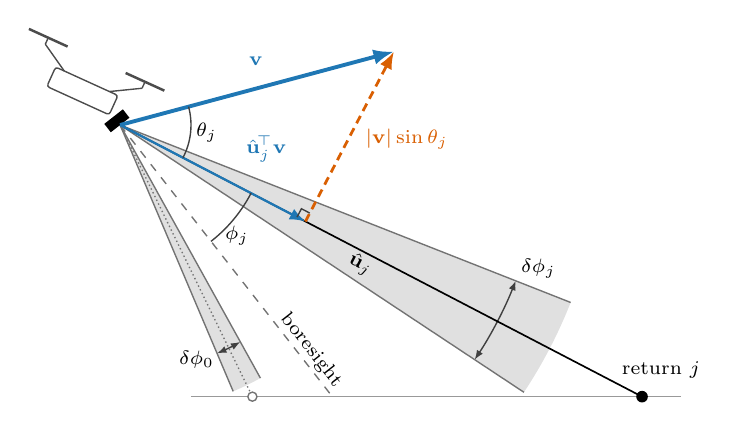
\begin{tikzpicture}[
  scale=1.5,
  font=\footnotesize,
  supp/.style={black!55, line width=0.5pt},
  scene/.style={black!40, line width=0.5pt},
  ray/.style={black!55, line width=0.5pt, densely dotted},
  rayj/.style={black, line width=0.6pt},
  wedge/.style={fill=black!12, draw=none},
  vel/.style={-{Latex[length=2.6mm]}, line width=1.4pt, geoblue},
  velpar/.style={-{Latex[length=2.0mm]}, line width=0.8pt, geoblue},
  velperp/.style={-{Latex[length=2.2mm]}, line width=1.0pt, geoorange, densely dashed},
  ang/.style={black!75, line width=0.5pt},
  lbl/.style={font=\scriptsize},
]
\definecolor{geoblue}{RGB}{31,119,180}
\definecolor{geoorange}{RGB}{217,95,2}
% side view; the radar is at S, the body is pitched 24.5 deg nose down
% (dynamic flight), the boresight a further 27.5 deg down: -52 deg
\coordinate (S) at (0,0);
% static scene: floor and a wall ahead
\draw[scene] (0.6,-2.3) -- (4.75,-2.3);
% bearing cones: they swing the ray about the radar and do not stretch it
\fill[wedge] (S) -- (-33.5:4.1) arc (-33.5:-21.5:4.1) -- cycle;
\fill[wedge] (S) -- (-67:2.45) arc (-67:-61:2.45) -- cycle;
\draw[supp] (S) -- (-33.5:4.1);  \draw[supp] (S) -- (-21.5:4.1);
\draw[supp] (S) -- (-67:2.45);   \draw[supp] (S) -- (-61:2.45);
\draw[ang, {Latex[length=1.2mm]}-{Latex[length=1.2mm]}] (-33.5:3.6) arc (-33.5:-21.5:3.6);
\draw[ang, {Latex[length=1.2mm]}-{Latex[length=1.2mm]}] (-67:2.1) arc (-67:-61:2.1);
\node[lbl, anchor=south west, inner sep=1pt] at (-21.5:3.62) {$\delta\phi_j$};
\node[lbl, anchor=east, inner sep=1pt] at (-67.5:2.15) {$\delta\phi_0$};
% the near-boresight return (static scene point on the floor)
\draw[ray] (S) -- (1.12,-2.30);  \draw[supp, fill=white] (1.12,-2.30) circle (1.1pt);
% return j: a floor point ahead, 24.5 deg above the boresight
\draw[rayj] (S) -- (4.419,-2.30); \fill (4.419,-2.30) circle (1.4pt);
\node[lbl, anchor=south west, inner sep=1pt] at (4.22,-2.17) {return $j$};
\node[lbl, rotate=-27.5, anchor=north, inner sep=1pt] at (-27.5:2.35) {$\vu_j$};
% radar boresight (sensor x), stops at the floor
\draw[supp, dashed] (S) -- (-52:2.9);
\node[lbl, rotate=-52, anchor=south east, inner sep=1pt] at (-52:2.9) {boresight};
% quadrotor icon (side view), pitched nose down, radar at the nose underside
\begin{scope}[rotate=-24.5]
\draw[black!70, line width=0.5pt, fill=white, rounded corners=1pt] (-0.70,0.04) rectangle (-0.12,0.22);
\draw[black!70, line width=0.5pt] (-0.62,0.22) -- (-0.86,0.36) (-0.20,0.22) -- (0.04,0.36);
\draw[black!70, line width=0.5pt] (-0.86,0.36) -- (-0.86,0.42) (0.04,0.36) -- (0.04,0.42);
\draw[black!70, line width=0.9pt] (-1.04,0.42) -- (-0.68,0.42) (-0.14,0.42) -- (0.22,0.42);
\end{scope}
% the radar: a thin plate at the nose whose face normal IS the boresight
\begin{scope}[rotate=-52]
\fill[black] (-0.09,-0.10) rectangle (0.0,0.10);
\end{scope}
% velocity (15 deg, length 2.4) and its decomposition on ray j
\draw[vel] (S) -- (15:2.4);
\node[lbl, geoblue, anchor=south] at (1.15,0.42) {$\vv$};
\draw[velpar] (S) -- (-27.5:1.769);
\node[lbl, geoblue, anchor=west, inner sep=0.5pt] at (1.05,-0.20) {$\vu_j^{\!\top}\vv$};
\draw[velperp] (-27.5:1.769) -- (15:2.4);
\node[lbl, geoorange, anchor=west, inner sep=1pt] at (2.05,-0.12) {$|\vv|\sin\theta_j$};
\draw[ang] ($(-27.5:1.769)+(62.5:0.08)$) -- ($(-27.5:1.769)+(62.5:0.08)+(152.5:0.08)$) -- ($(-27.5:1.769)+(152.5:0.08)$);
% the two angles on the same ray: theta against v (above), phi against the boresight (below)
\draw[ang] (-27.5:0.60) arc (-27.5:15:0.60);
\node[lbl, anchor=west, inner sep=0.5pt] at (-6:0.63) {$\theta_j$};
\draw[ang] (-52:1.25) arc (-52:-27.5:1.25);
\node[lbl, anchor=west, inner sep=0.5pt] at (-47:1.28) {$\phi_j$};
\end{tikzpicture}
\caption{Geometry behind the per-return law (Eq.~\eqref{eq:law}) in side view.
The platform moves with velocity $\vv$ past static scene points.  Return $j$ is the ray of direction $\vu_j$ from the radar to one of them.  The sensor reads only the along-ray part of the velocity, the Doppler $v_{D}=-\vu_j^{\top}\vv$ (positive for a receding target, so negative here).
A bearing error swings the ray about the radar (grey cones) and leaves its length unchanged, so to first order it projects only the transverse velocity, of magnitude $|\vv|\sin\theta_j$, into the Doppler residual.  $\theta_j$ is the angle between the ray and $\vv$.
The angular width of the cone grows off the boresight (dashed: the sensor $x$ axis, mounted $27.5\degree$ below the body's forward axis), from about $\delta\phi_0$ near the boresight to $\delta\phi_j = \delta\phi_0/\cos\phi_j$ at the off-boresight angle $\phi_j$.  This widening follows from the angle FFT's uniform binning in the direction cosine $\sin\phi$.}
\label{fig:geometry}
\end{figure}

\textbf{Derivation.}  Bearing error provides a model for these three
trends.  We derive it first in the angular form of
\autoref{fig:geometry}; the deployed weight uses the direction-cosine
form of the same law (\autoref{sec:robust}).  The sensor measures radial velocity along the \emph{true}
ray, $v_{\mathrm{meas}} = -\vu_{\mathrm{true}}^\top\vv$, while the
forward model predicts with the \emph{reported} ray,
$v_{\mathrm{pred}} = -\vu_{\mathrm{rep}}^\top\vv$.  The residual due to
the direction error $\delta\vu = \vu_{\mathrm{rep}} - \vu_{\mathrm{true}}$
is $r_j = \delta\vu^\top\vv$.  Both rays are unit vectors, so to first
order $\delta\vu$ is perpendicular to the ray, and only the transverse
velocity $\vv_\perp$, of magnitude $|\vv|\sin\theta_j$, couples into
the residual, $r_j \approx \delta\vu^\top\vv_\perp$.  For isotropic
tangent-plane error with total angular rms $\delta\phi_j$ across its
two components, the component along $\vv_\perp$ has rms
$\delta\phi_j/\sqrt2$.  The angle FFT uses uniformly
spaced bins in the \emph{direction cosine} $\sin\phi$.
Differentiating $\sin\phi$ converts
a constant direction-cosine error into the angle error
$\delta\phi_j = \delta\phi_0/\cos\phi_j$.  The bearing-error contribution is therefore
\begin{equation}
  \sigma_j = \frac{\delta\phi_0}{\sqrt2}\,
             \frac{|\vv|\sin\theta_j}{\cos\phi_j},
  \label{eq:law}
\end{equation}
which captures the speed and geometry dependence.  Each return also
contains speed-independent noise, including detection and quantization
noise.  Independent sources add in
variance, so with $q_j = |\vv|\sin\theta_j/\cos\phi_j$ the total variance
is modeled as
\begin{equation}
  \sigma_j^2 = \sigma_0^2 + (c\,q_j)^2, \qquad c = \delta\phi_0/\sqrt2,
  \label{eq:law_fit}
\end{equation}
with a noise floor $\sigma_0$ and coefficient $c$.  The deployed weight
uses the direction-cosine form in \eqref{eq:dircos}
(\autoref{sec:robust}), assigning constant error to the two resolved
cosines and fixing the third by unit norm.  The constants reported
below are fitted to that form.

\textbf{Fit and test.}  Fitted to the binned robust width of the
per-return deviations on the two racing flights (10 quantile bins per
flight, one shared coefficient and a per-flight floor), the law
reproduces the binned widths with $R^2 = 0.98$.  The
normalized deviations $d_j/\sigma_j$ provide a further check:
their robust width should be approximately 1 across bins of each input
(\autoref{fig:law}d).  The full law gives approximately flat profiles;
omitting a factor leaves a trend along the corresponding input.
The transverse factor shows
the smallest effect in \autoref{fig:law}d because most racing returns
have $\sin\theta \ge 0.5$ (73--80\%); it is retained
because it follows from the bearing-error model and improves the fit
($R^2 = 0.98$ against
$0.93$ without).  Held out of the fit, the
backflip flight keeps this width near 1 along speed and $\theta$,
but excess noise remains off boresight.
Additional terms fitted jointly to the same statistic receive zero
coefficients, including the body-rate term.  Thus body rate adds no
explanatory value to this fit after accounting for speed and geometry.

\textbf{Constants.}  Fitting the racing flights gives
$\delta\phi_0 = 2.7\degree$; adding the backflip flight with its own
floor changes this estimate by 3\%, supporting a shared coefficient.
The firmware uses 64 direction-cosine bins over the field of view;
the fitted error corresponds to approximately one bin per axis.
The noise floor varies across regimes
($\sigma_0 = 0.049/0.140/0.327$\,m/s on the three flights,
\autoref{tab:char}), collecting the speed-independent errors the law
does not model.  Possible sources include detection noise, smearing
at high body rate, and errors near the aliasing boundary.
A shared floor would confound these differences with the bearing-error
coefficient.  The solver uses the geometric mean of the two racing
floors, $\sigma_0 = 0.083$\,m/s, and
\autoref{sec:ablations} measures the sensitivity to that choice.

\emph{Consequence.}  Each return receives its own weight,
$w_j = \sigma_0^2/\sigma_j^2 = 1/(1 + (c\,q_j/\sigma_0)^2)$, from its
own geometry and the frame's speed; the weight halves at
$q_j = \sigma_0/c = 2.5$\,m/s.  Speed is obtained from the frame's
consensus ego-velocity.  The \ac{imu} is used in the radar front end
only for alias unwrapping (\autoref{sec:robust}).
The fitted model does not include a body-rate term.

\begin{figure*}[t]
  \centering
  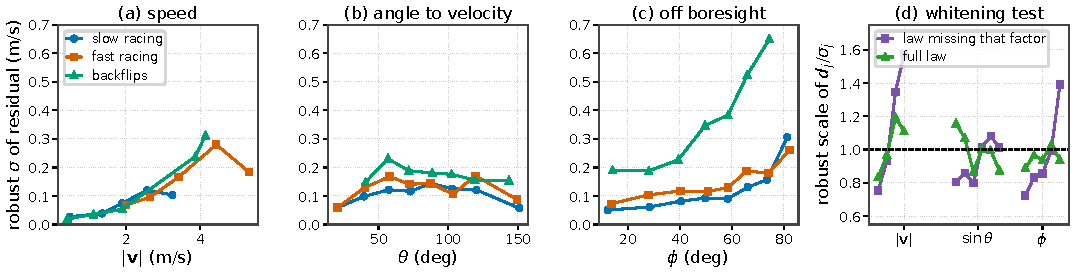
\includegraphics[width=\textwidth]{figures/law.pdf}
  \caption{The per-return noise law.  (a--c)~Robust width of the
    within-frame deviations binned by platform speed $|\vv|$, by the angle
    $\theta$ between ray and velocity, and by the angle $\phi$ off
    boresight, for the three flights: the three trends of
    \eqref{eq:law} are visible before fitting.  (d)~Model check on fast
    racing: robust scale of the normalized deviation
    $d_j/\sigma_j$ binned along each input, for the full law (green)
    and the law missing the corresponding factor (purple).  The expected
    scale is approximately 1; each missing factor leaves a trend along its
    own input.}
  \label{fig:law}
\end{figure*}

\subsection{Frame-Shared Error}
\label{sec:char_corr}
The returns of one frame share a timestamp, an attitude and an
integration interval, which can introduce correlated errors.
We estimate a frame-shared component $\sigma_c$ by separating
within-frame variation from variation in the frame means.
In units of the noise floor $\sigma_0$ of the deployed law,
$\sigma_c = 0.96/1.38/1.55$ on slow racing, fast racing
and backflips, and $0.83$--$1.02$ on the four public ICINS flights
(\autoref{sec:baselines}): the shared component is of the same order
as the per-return noise and increases across our three flight regimes.
This correlation reduces the effective number of independent
returns~\cite{kish1965survey}.

\emph{Consequence.}  Treating the returns of a frame as independent
would overstate the information in their shared component.
The estimator includes this component in the frame covariance and
whitens the residual stack as described in \autoref{sec:robust}.
We use $\sigma_c = 1.27$, the geometric mean over our three flights,
for every platform.

\subsection{Aliasing}
\label{sec:char_alias}
The firmware wraps Doppler into $\pm v_{\max} = \pm3.14$\,m/s.  Measured
against ground truth, 2.0\% of returns are aliased on slow racing,
23.7\% on fast racing and 37.8\% on backflips.
Unwrapping recovers the Doppler ambiguity but does not correct bearing
errors.  At matched speed, aliased returns have within-frame noise
2--4.6$\times$ that of non-aliased returns, with a noise floor of
$\sigma_{\mathrm{al}} \approx 0.6$\,m/s and weaker state dependence.

\emph{Consequence.}  The measurement consumed by the estimator is the
\emph{unwrapped} Doppler, selected once per frame against an
\ac{imu}-integrated velocity prediction (\autoref{sec:init}).  Selecting
the correct wrap requires the predicted radial velocity to be within
$v_{\max}$ of the true value.  Aliased returns are retained with the
reduced weight given by the measured
variance ratio $w_{\mathrm{al}} = (\sigma_0/\sigma_{\mathrm{al}})^2 = 0.019$;
\autoref{sec:results} compares this choice with full weighting and deletion.

\subsection{Doppler Residual Distribution}
\label{sec:char_noise}
A zero-mean Gaussian error model with the specified covariance yields
a covariance-weighted least-squares likelihood.  The raw residuals have
an approximately Gaussian core but heavy tails (\autoref{fig:ladder}a).
The front end treats aliased returns separately
(\autoref{sec:char_alias}) and rejects consensus outliers
(\autoref{sec:char_outliers}).  Normalizing each retained return by its
own $\sigma_j$ (\autoref{sec:char_rate}) reduces the excess mass between
$1.5\sigma$ and $3\sigma$, while the prefilter reduces the far tail
(\autoref{fig:ladder}b).

For the retained, non-aliased returns, the mass beyond $3\sigma$ is
3--10$\times$ the Gaussian value, down from
25--47$\times$ before the prefilter with one global $\sigma$.  The
remaining outlier population is not identified by the available flags:
it accounts for 1--4\% of the returns and is
5--10$\times$ wider than the core, against 6--12\% and 6--11$\times$
before.  Multipath is a possible source.  The residuals remain
approximately zero-mean and symmetric, with tails consistent with
exponential decay over the observed range.

\emph{Consequence.}  We use a Gaussian likelihood with per-return
variance $\sigma_j^2$ and frame-shared covariance
(\autoref{sec:prelim_map}, \autoref{sec:robust}).  This approximates the
core but does not model the remaining heavy tails.  A robust kernel
after prefiltering produced no measurable improvement and is not used
(\autoref{sec:ablations}).

\begin{figure*}[t]
  \centering
  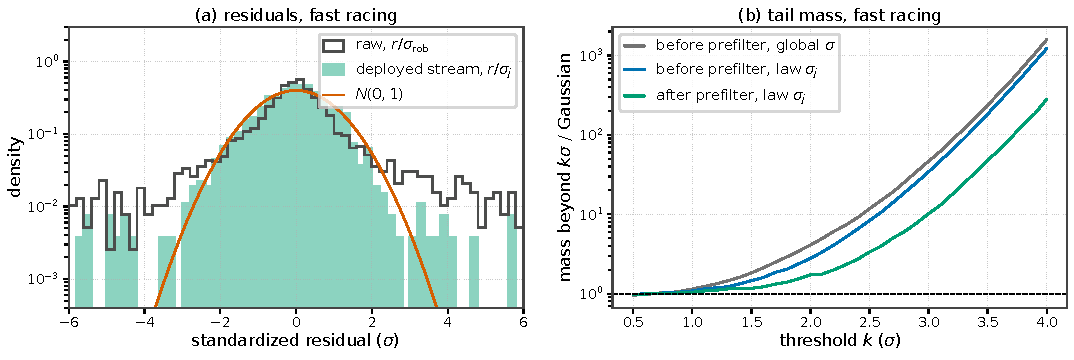
\includegraphics[width=\textwidth]{figures/ladder.pdf}
  \caption{The residual distribution before and after the front end
    (fast racing).  (a)~Standardized residuals on a log density scale:
    the raw stream in units of its $\sigma_{\mathrm{rob}}$ (grey) and
    the retained, non-aliased returns, each residual in units of its own
    $\sigma_j$ (green), against $N(0,1)$.  Aliased returns are weighted
    as their own population and are not in the green stream.
    (b)~Tail mass beyond $k\sigma$ relative to a Gaussian, for the
    non-aliased returns before the prefilter with one global $\sigma$
    (grey) and with the per-return law $\sigma_j$ (blue), and for the
    returns after the prefilter with the law (green).  Together they
    reduce the excess by an order of magnitude.  Per-return normalization
    mainly reduces the excess between $1.5\sigma$ and $3\sigma$;
    the blue and grey curves converge beyond $3.5\sigma$.
    The prefilter reduces the remaining far tail.}
  \label{fig:ladder}
\end{figure*}

\subsection{Stream Error Budgets}
\label{sec:char_budget}
The noise law sets the relative weights of radar returns.  The weights
of the radar, gyroscope, and accelerometer streams must also account
for temporal correlation.  We approximate a stream sampled at $f_s$ with integrated
autocorrelation time $\tau$ (the sum of the residual autocorrelation
over positive lags) as providing $1/\tau$ independent samples per
second.  The corresponding per-sample weight is
\begin{equation}
  \lambda^\ast = \frac{1}{\sigma^2\, f_s\, \tau},
  \label{eq:lambda_star}
\end{equation}
which for white noise ($\tau = 1/f_s$) reduces to
$1/\sigma^2$ per sample.  Both inputs are measured per stream against
the reference.  For the \ac{imu}, we use residuals within the bandwidth
represented by the splines.  Much of the raw residual energy lies above
this band: the gyroscope's in-band $\sigma$ is 0.024--0.051\,rad/s,
compared with 0.15\,rad/s before filtering.  The measured \ac{imu}
correlation times are 194--598\,ms, corresponding to approximately
2--5 independent samples per second under this approximation.
For the radar, $\sigma$ is the root-mean-square residual of the
non-aliased returns that pass the prefilter; aliased returns have their
own weight and are excluded from this estimate.  The second moment
includes the remaining outliers' contribution to the quadratic cost.
Using the robust core width instead makes the weights from the two
racing flights differ by a factor of $3.6$.

\emph{Consequence.}  Taking the geometric mean of
\eqref{eq:lambda_star} over the two racing flights gives
$\lambda_g = 3.13$, $\lambda_a = 0.0039$, and a radar weight of $2.64$
per return (\autoref{sec:robust}).  Ignoring temporal correlation would
increase the \ac{imu} weights by $f_s\tau$, a factor of several hundred,
relative to this approximation.  \autoref{sec:nees} tests the consistency
of the resulting estimator covariance.

\section{Methodology}
\label{sec:method}

\subsection{State Representation}
\label{sec:state}

\textbf{Position.}
The world-frame position $\vp_w(t) \in \mathbb{R}^3$ is a quintic
(order-6) uniform B-spline with knot spacing $\Delta t_p = 40$\,ms.
Velocity $\dot{\vp}_w$ and acceleration $\ddot{\vp}_w$ are
obtained as analytical derivatives of the spline.

\textbf{Orientation.}
The body-to-world rotation $\vR(t)=\vR_{wb}(t)$ is a cubic
cumulative $\SO$ B-spline~\cite{sommer2020efficient,usenko2020basalt}:
\begin{equation}
  \vR(t) = \vR_{k-3}
           \prod_{j=k-2}^{k} \Exp\!\bigl(\tilde{B}_j(t)\,
           \Log(\vR_{j-1}^{-1}\vR_{j})\bigr),
  \label{eq:ori_spline}
\end{equation}
where $\vR_{k-3},\ldots,\vR_k$ are the four active orientation control points
and $\tilde{B}_j(t)$ are the cumulative basis functions defined in
\autoref{sec:prelim_so3}.  The absolute orientation control points are optimized.
The knot spacing is $\Delta t_o = 16$\,ms, and the body-frame angular
velocity $\vom_b(t)$ follows by analytic differentiation.
Both spline spacings are fixed across flights and platforms
(\autoref{sec:negative}).

\textbf{Biases and extrinsics.}
The constant six-component \ac{imu} bias $[\vb_a,\vb_g]$ is estimated
jointly with the trajectory.  A Gaussian prior anchors it to the
stationary initialization (\autoref{sec:init}), with standard
deviations $0.216$\,m/s$^2$ and $0.0036$\,rad/s for the accelerometer
and gyroscope, respectively.  These widths are measured offline from stationary ground segments,
the accelerometer's against the specific force $-\vR_{bw}\vg_w$
predicted from the \ac{mocap} attitude, the gyroscope's from the
bias shift between motors off and motors running.  The prior weights are inverse variances, and the prior touches no leaving state, so it is re-applied in every window and never absorbed into the marginalization prior (\autoref{sec:sw}).
All radar extrinsics are fixed at the platform's measured values.
On our platform, freeing the pitch left the estimate close to its
initial value, so we use the measured $27.5\degree$ mount angle
(\autoref{sec:overview}).

\subsection{Measurement Models}
\label{sec:models}

\textbf{Radar Doppler with lever arm.}
For a static target at sensor-frame bearing $\vu_s$, the predicted
Doppler is
\begin{equation}
  v_D = -\vu_b^{\top}\!\left(
    \vR_{bw}\,\vv_w(t) + \vom_b(t) \times \mathbf{t}_{bs}
  \right),
  \label{eq:doppler}
\end{equation}
where $\vv_w=\dot{\vp}_w$, $\vu_b=\vR_{bs}\vu_s$,
$\vR_{bs}$ rotates sensor coordinates into the body frame, and
$\vR_{bw}=\vR_{wb}^{\top}$.  The lever arm $\mathbf{t}_{bs}$ runs
from the body \ac{com} to the radar antenna, expressed in body coordinates.
The sign follows the sensor convention: positive Doppler denotes a
receding target.  Each return contributes a residual
$r_{f,j}=v_{D,\mathrm{meas}}-v_{D,\mathrm{pred}}$ to its frame's
jointly weighted residual block (\autoref{sec:robust}).

\textbf{Accelerometer.}
\begin{equation}
  \mathbf{r}_a = \vz_a - \vR_{bw}\!\left(\ddot{\vp}_w - \vg_w\right) - \vb_a,
  \label{eq:accel}
\end{equation}
where $\vz_a$ is the measured specific force and $\vg_w$ is gravity
in world coordinates.

\textbf{Gyroscope.}
\begin{equation}
  \mathbf{r}_g = \vz_g - \vom_b(t) - \vb_g,
  \label{eq:gyro}
\end{equation}
Here $\vz_g$ is the measured body-frame angular rate.  The weights
for both \ac{imu} residuals are specified in \autoref{sec:robust}.

\textbf{Heading prior.}
Absolute yaw is unobservable from Doppler and \ac{imu} measurements:
a common rotation of position, velocity and attitude about gravity
leaves these measurements unchanged.  We supply heading using
\ac{mocap} yaw at approximately 100\,Hz as an idealized magnetometer
surrogate.  With $\mathbf{h} = \vR\,\mathbf{e}_x$ the body forward axis in world
coordinates, the residual is
\begin{equation}
  r_\psi = h_x \sin\psi_{\mathrm{ref}} - h_y \cos\psi_{\mathrm{ref}},
  \label{eq:heading}
\end{equation}
i.e.\ $\sin(\psi-\psi_{\mathrm{ref}})$ scaled by the horizontal
projection of the forward axis, with weight $\lambda_\psi=0.6$.  It
needs no angle wrapping, vanishes when the nose points vertically (the
heading is momentarily undefined through a flip), and has a spurious
zero at the opposite heading, which the initialization avoids.
\autoref{sec:yaw} discusses this weight and the limitations of the surrogate.

\subsection{Radar Front End and Measurement Weighting}
\label{sec:robust}

The radar front end unwraps Doppler, rejects consensus outliers and
assigns weights before optimization.  The measurement characterization
in \autoref{sec:char} motivates these steps.

\textbf{Alias unwrapping and the alias weight.}
At frame load, each return's Doppler alias is selected using the
radial velocity predicted from \ac{imu} integration
(\autoref{sec:init}).  Correct selection requires the predicted radial
velocity to be within $v_{\max}$ of the true value.  All subsequent
stages use this unwrapped Doppler.
Unwrapping does not correct the bearing errors of aliased returns.
These returns retain their reported bearings but receive the reduced
weight $w_{\mathrm{al}}=0.019$, the measured ratio of clean to aliased
noise-floor variances (\autoref{sec:char_alias}).

\textbf{Consensus prefilter.}
Following \mbox{reve}~\cite{doer2020ekf}, three-point \ac{ransac}
estimates ego-velocity for each frame.  Only returns within
$0.15$\,m/s of the consensus prediction reach the solver
(\autoref{sec:char_outliers}).  Frames with fewer than five returns
bypass this filter.  Filtering runs once at frame load.

\textbf{Per-return weights in the frame covariance.}
For each retained, non-aliased return, the relative inverse-variance
weight from \eqref{eq:law_fit} is, in the simplified angular model,
\begin{equation}
  w_{f,j} = \frac{1}{1 + (c\,q_{f,j}/\sigma_0)^2}, \qquad
  q_{f,j} = \frac{\lVert\vv_f\rVert\sin\theta_j}{\cos\phi_j},
  \label{eq:weight}
\end{equation}
where $\theta_j$ is the angle between velocity and ray, and $\phi_j$
is the angle off boresight.  The constants are
$c=\delta\phi_0/\sqrt2$, $\delta\phi_0=2.7\degree$ (converted to
radians), and $\sigma_0=0.083$\,m/s (\autoref{sec:char_rate}).
The solver uses the direction-cosine form of the same law: with
$\mathbf{s}$ the unit bearing and $\vv_s$ the frame velocity, both in
sensor coordinates, and $c_\phi = \max(s_x, 0.15)$,
\begin{equation}
\begin{aligned}
  X_j &= \sqrt{(v_{s,y} - s_y v_{s,x}/c_\phi)^2 + (v_{s,z} - s_z v_{s,x}/c_\phi)^2},\\
  \sigma_j^2 &= \sigma_0^2 + (c\,X_j)^2,
\end{aligned}
\label{eq:dircos}
\end{equation}
which needs no clamp towards $\phi = 90\degree$ beyond the floor on
$c_\phi$; $w_{f,j} = \sigma_0^2/\sigma_j^2$.
The velocity $\vv_f$ comes from the frame's \ac{wls} consensus fit.
Weights are fixed when the problem is built, independently of later
trajectory updates.  They still depend on the \ac{imu} prediction
through the earlier alias decisions.

The residuals of frame $f$ are stacked in $\mathbf{r}_f$.  Their
covariance model is
\begin{equation}
  \Sigma_f = \sigma_0^2\!\left[
    \mathrm{diag}(w_{f,j}^{-1})
    + \sigma_c^2\mathbf{1}\mathbf{1}^{\top}\right],
  \label{eq:frame_cov}
\end{equation}
using $w_{f,j}=w_{\mathrm{al}}$ for aliased returns and
$\sigma_c=1.27$ for the shared component (\autoref{sec:char_corr}).
The rank-one term accounts for a common additive error within a frame,
reducing the information attributed to repeated observations of that
component.  The frame is weighted jointly, as specified below.

\textbf{Accelerometer gate.}
The accelerometer weight decreases with body-rate magnitude to limit
the influence of vibration and other unmodeled high-dynamic errors.
The gate in \eqref{eq:comp_a} uses an empirical scale
$\omega_a=8$\,rad/s, chosen from the velocity--orientation trade-off.
Translational acceleration itself is already included in
\eqref{eq:accel}.  The gyroscope weight remains constant.

\textbf{Static stream weights.}
The per-sample stream weights follow the correlation-adjusted error
budgets of \eqref{eq:lambda_star}.  Taking their geometric means over
the two racing flights gives $\lambda_g=3.13$, $\lambda_a=0.0039$
and $\lambda_r=2.64$.  These weights are fixed across flights and
platforms.

\textbf{The complete weighting.}
The effective information weights are
\begin{align}
  \Lambda^{\mathrm{gyro}}  &= \lambda_g, \label{eq:comp_g}\\
  \Lambda^{\mathrm{accel}} &= \frac{\lambda_a}{1 + (\lVert\vom_b\rVert/\omega_a)^2}, \label{eq:comp_a}\\
  \Lambda^{\mathrm{radar}}_f &= \lambda_r\,\sigma_0^2\Sigma_f^{-1}. \label{eq:comp_r}
\end{align}
Thus the radar contribution is
$\sum_f\mathbf{r}_f^{\top}\Lambda^{\mathrm{radar}}_f\mathbf{r}_f$.
The factor $\sigma_0^2$ normalizes the covariance because $\lambda_r$
already includes the stream's inverse-variance scale.  Without
within-frame correlation, this reduces to
$\lambda_r\sum_{f,j}w_{f,j}r_{f,j}^2$.
All retained measurement residuals enter quadratically, without a
robust kernel.  The constants in these weights are measured except
for the empirical accelerometer gate.

\subsection{Regularization}
\label{sec:reg}

\textbf{Position: minimum snap.}
$E_{\text{snap}} = \lambda_s \sum_i \|\vp^{(4)}(t_i + \Delta t_p/2)\|^2$,
one term per knot interval (the midpoint sum of the snap integral,
without the $\Delta t_p$ factor), with $\lambda_s = 2{\times}10^{-5}$.

\textbf{Orientation: angular-increment smoothness.}
We penalize changes between consecutive rotation increments:
\begin{equation}
  \mathbf{r}_\alpha = \Log(\vR_{i-1}^{-1}\vR_i)
                    - \Log(\vR_i^{-1}\vR_{i+1}),
  \label{eq:min_alpha}
\end{equation}
The cost is $\lambda_\alpha\sum_i\lVert\mathbf{r}_{\alpha,i}\rVert^2$
with $\lambda_\alpha=0.1$.  This discrete smoothness penalty is zero
for equal consecutive increments.  It approximates angular-acceleration
regularization at the fixed knot spacing but is not a time-normalized
angular-acceleration residual.  Both regularization weights are design
choices (\autoref{sec:fixed_constants}).

\subsection{Sensor-Only Initialization (P1--P3)}
\label{sec:init}

\textbf{P1: Orientation.}
An automatically detected stationary segment provides the mean
gyroscope bias and a gravity-aligned scalar accelerometer correction.
This does not identify the full accelerometer bias independently of
tilt.  Initial roll and pitch follow from the corrected gravity
direction, and yaw is set to zero until heading aiding is applied.
Orientation is initialized by integrating debiased gyroscope readings:
$\vR(t+\Delta t) = \vR(t)\,\Exp\!\bigl((\vz_g - \vb_g)\Delta t\bigr)$.

\textbf{P2: Position.}
The front end of \autoref{sec:robust} produces a per-frame \ac{wls}
ego-velocity estimate from the unwrapped, prefiltered returns.
Rotated into the world frame with the initialized attitude (the lever
arm is neglected at this stage), it is integrated with forward Euler
into the initial position trajectory.  The alias predictor of
\autoref{sec:robust} is the \ac{imu}-integrated velocity from the same
attitude, and a frame whose consensus fails keeps all its returns.

\textbf{P3: Boundary priors.}
Position, velocity and orientation priors anchor the first window at
$t=0$ to the initialized state, with hand-set weight
$\lambda_{\text{bnd}}=1000$.  They are not re-applied in later windows,
which carry previous information through the marginalization prior
(\autoref{sec:sw}).

\subsection{Sliding Window with Marginalization}
\label{sec:sw}

The fixed-lag smoother advances a 3\,s window in 0.3\,s strides.
After each solve, position and orientation control points leaving the
window are eliminated from the linearized problem by a Schur
complement.  The retained variables coupled to these states, including
the shared bias, form the boundary of the next window.  The resulting
information matrix is stored as a Gaussian prior, with the
approximations described below.

\textbf{Which factors enter the marginal.}
Factors touching a leaving variable, including the previous prior
when applicable, enter the Schur complement and are then removed from
the active problem.  Factors involving only retained variables remain
active and must not also be absorbed into the prior.  In particular,
sharing the retained \ac{imu} bias does not justify including every
\ac{imu} factor.  The boundary is the last five position control points and three
orientation control points before the window start, plus the bias (30
coordinates).  A factor touching a leaving variable whose support
would reach past this boundary, a sliver at the mismatch of the two
grids, is dropped rather than absorbed, so the prior stays a marginal
over exactly that boundary.

\textbf{Re-centered prior.}
Before each solve, the prior is centered at the current warm start
$\mathbf{x}_0$, retaining its information matrix and setting its
gradient there to zero.  This is a curvature-only approximation to
the marginalized problem.  It generally changes the prior's mean,
so it does not preserve the full Gaussian marginal.  The prior still
penalizes subsequent departures from the warm start during the solve.

\textbf{Staleness of the prior.}
To reduce reliance on older linearizations during rotation, the
prior's position and orientation uncertainties are increased with
accumulated angular travel.  The update adds the variance $(k\theta)^2$ to every boundary position
and orientation coordinate of the marginal's covariance (a Woodbury
update, so the cross-covariances follow), with $\theta$ the rotation
accumulated over the marginalized stride and the rates $k = 0.12$\,m
and $0.01$\,rad per radian measured as the live-edge position and
orientation error increments per swept radian against ground truth
(the position rate is $0.12$, $0.12$ and $0.17$\,m/rad on the three
flights).  Angular travel is a proxy for linearization error, not a
direct measure of it.
Apart from this inflation, no global scale factor is applied to the
prior.  \autoref{sec:ablations} evaluates the effect of position
inflation, and \autoref{sec:nees} tests the output covariance.

\textbf{Live-edge warm start.}
The incoming trajectory segment is aligned to the previous solution
at its last data-supported position and orientation control points.  This
reduces mismatch at the transition before optimization.

\section{Experimental Setup}
\label{sec:setup}

\textbf{Datasets.}  \autoref{tab:datasets} summarizes the three
flights used for characterization and the main evaluation, recorded
as rosbags in a Vicon \ac{mocap} lab on the platform described in
\autoref{sec:overview}.  Additional held-out flights
(\autoref{sec:heldout}) and four public ICINS-2021 flights with
VINS pseudo ground truth (\autoref{sec:baselines}) test transfer
beyond these recordings.

\begin{table}[t]
\centering
\caption{Dataset Summary}
\label{tab:datasets}
\small
\begin{tabular}{@{}lcccc@{}}
\toprule
Flight & Dur.\ (s) & $v_{\max}$ (m/s) & $|\omega|_{\max}$ (rad/s) & Frames \\
\midrule
Slow racing & 25.8 & 3.65 & 2.62 & 258 \\
Fast racing & 18.0 & 5.66 & 9.14 & 179 \\
Backflips\textsuperscript{*} & 18.1 & $\sim$4.3 & $\sim$10.9 & 181 \\
\bottomrule
\multicolumn{5}{@{}p{\columnwidth}@{}}{\scriptsize \textsuperscript{*}Backflip
speed and angular rate are 95th percentiles rather than maxima because
\ac{mocap} tracking artifacts dominate the instantaneous peaks.}
\end{tabular}
\end{table}

\textbf{Configuration.}  Unless varied in an ablation, all flights
on both platforms use the configuration of \autoref{sec:method}:
a 3\,s window, 0.3\,s stride, and knot spacings
$\Delta t_p=40$\,ms and $\Delta t_o=16$\,ms, with no per-flight
retuning.  Radar extrinsics are fixed at each platform's
calibration, measured on ours and published with the public
dataset.  Nothing else was re-measured for the second platform: the noise-model
constants and stream weights are those measured on our own sensor and
flights (\autoref{sec:char}); the per-sample \ac{imu} weights were
applied unchanged at its 409\,Hz rate, and \autoref{sec:baselines}
reports what that costs.  Initialization uses radar and \ac{imu}
alone; heading aiding uses reference yaw as an idealized
magnetometer surrogate with $\lambda_\psi=0.6$ (\autoref{sec:yaw}).

\textbf{Evaluation.}  The reference is \ac{mocap} on our flights and the
public dataset's pseudo ground truth on theirs.
Estimates are aligned to the reference by the
rigid transform at the first frame only, without scale correction or
a whole-trajectory fit.  Such a fit is common in odometry work and is the
weaker protocol, since it can absorb accumulated drift into the transform.
The final 3\,s is excluded from evaluation.
Velocity \ac{rmse} compares the spline's analytical derivative with
the low-pass filtered reference velocity.  \emph{Position drift}
denotes position \ac{rmse} divided by the reference path length,
expressed as a percentage.  The \emph{live} \ac{rmse} uses each
window's newest stride before subsequent refinement; the
\emph{settled} \ac{rmse} uses the trajectory after all windows have
refined it.  For comparison with published results,
\autoref{tab:baselines}(b) additionally reports the whole-trajectory
\ac{ate} under Umeyama alignment.
\section{Results}
\label{sec:results}

\subsection{Live-Edge Results}
\label{sec:sw_results}

\autoref{tab:sw} reports live-edge and settled errors for the three
flights using the configuration in \autoref{sec:setup}.
\autoref{fig:traj} and \autoref{fig:error_time} show the trajectories
and live-edge errors.  We report velocity first because Doppler
constrains it directly.  Position is its integral.

\begin{table}[t]
\centering
\caption{Sliding Window: Live Leading-Edge and Settled \ac{rmse}
  (per-window solve time on a laptop CPU)}
\label{tab:sw}
\small
\setlength{\tabcolsep}{3pt}
\begin{tabular}{@{}llcccc@{}}
\toprule
Flight & Mode & Vel (m/s) & Ori (\degree) & Drift (\%) & $t_{\mathrm{win}}$ (s) \\
\midrule
\multirow{2}{*}{Slow racing}
  & \textbf{Live edge} & \textbf{0.16} & \textbf{1.65} & \textbf{0.32} & \multirow{2}{*}{0.16} \\
  & Settled & 0.17\textsuperscript{$\ast$} & 1.16 & 0.29 & \\
\midrule
\multirow{2}{*}{Fast racing}
  & \textbf{Live edge} & \textbf{0.28} & \textbf{2.56} & \textbf{1.33} & \multirow{2}{*}{0.18} \\
  & Settled & 0.42\textsuperscript{$\ast$} & 2.41 & 1.28 & \\
\midrule
\multirow{2}{*}{Backflips}
  & \textbf{Live edge} & \textbf{1.66} & \textbf{12.1} & \textbf{2.91} & \multirow{2}{*}{0.20} \\
  & Settled & 1.72\textsuperscript{$\ast$} & 7.91 & 2.75 & \\
\bottomrule
\multicolumn{6}{@{}p{\columnwidth}@{}}{\scriptsize
  The \textbf{bold} live-edge rows are the deployment-relevant figures.
  $^\ast$The settled trajectory combines control points last optimized
  in different windows.  Disagreement between those solutions distorts
  its velocity near stride boundaries and inflates the settled velocity
  \ac{rmse}, while live velocity comes from each window's own spline.
  Path lengths 48.1 / 44.9 / 54.1\,m.  Repeated solver runs on the same
  recordings vary by $<$2\%.}
\end{tabular}
\end{table}

On the racing flights, velocity \ac{rmse} is $0.16$--$0.28$\,m/s and
position drift is $0.3$--$1.3\%$ of the path length.  Errors increase
on the backflip flight, with orientation \ac{rmse} reaching $12.1\degree$
(\autoref{sec:backflips}).  All three regimes solve faster than the
0.3\,s stride on a laptop CPU (\autoref{tab:sw}), i.e.\ the deployed
settings run in real time.

\begin{figure*}[t]
  \centering
  
\includegraphics[width=\textwidth]{figures/traj_combined.pdf}
  \caption{Trajectory overlays for all three flights (columns): \ac{mocap}
    ground truth vs.\ the sliding-window live edge, X--Y (top) and Y--Z
    (bottom) projections. Within each column both projections share a
    common $Y$ range and metric scale (equal aspect, so loops keep their
    true shape).  The scale differs between columns.  Start~$\blacksquare$.
    the dotted lead-in is the first window's estimate, available only
    once that window has been solved (the smoother needs one complete
    3\,s window), so it is not a live output at those timestamps.  It
    starts on the ground truth by the start-anchored alignment.
    The backflip flight circles in the horizontal plane while looping
    in the vertical plane.  Its position drifts through the flips
    ($2.9\%$ of the path) while the loops remain visible in the
    orientation estimate (\autoref{sec:backflips}).}
  \label{fig:traj}
\end{figure*}

\begin{figure*}[t]
  \centering
  
\includegraphics[width=\textwidth]{figures/error_over_time.pdf}
  \caption{Live-edge velocity, orientation, and position error (the last in percent of the flight's path length, the unit of the drift metric)
    vs.\ time for slow racing (top), fast racing (middle), and backflips
    (bottom).  Velocity and orientation errors spike at high-speed,
    high-dynamics sections.  Fast-racing position error accumulates with
    trajectory length.  Backflip errors grow step-wise \emph{during} the
    flips, where the radar measurement model degrades
    (\autoref{sec:backflips}).}
  \label{fig:error_time}
\end{figure*}

\subsection{Held-Out Validation}
\label{sec:heldout}
The per-return law and the stream weights were fitted on the two
racing flights with the backflip flight held out.  The frame-shared
term, the alias floor, the bias-prior widths and the staleness rates
were measured on all three.  The configuration was then run
\emph{unmodified} on flights never used for any decision.

A second, independent fast-racing flight was recorded with the radar's
on-chip clustering disabled (61 returns per frame instead of 11).  The
front end then collapses duplicate detections to the physical cluster
count, a preprocessing step that applies only when on-chip clustering
is off, with the solver configuration unchanged.  Velocity \ac{rmse}
is $0.27$\,m/s, compared with $0.28$\,m/s on the fitting flight.
Orientation \ac{rmse} is $2.7\degree$ and drift is $1.2\%$.
The four public ICINS flights in \autoref{sec:baselines} test
transfer to a different platform.

Accuracy degrades on a held-out circular flight at 5\,m/s.
With the radar's Doppler ambiguity of 3.1\,m/s, $63.8\%$ of its
returns must be
alias-unwrapped, the \ac{imu}-integrated unwrapper's alias decisions
degrade, and the live edge reaches
$1.30$\,m/s\,/\,$11.7\degree$\,/\,$9.1\%$.
Down-weighting aliased returns cannot compensate for incorrect wrap selection.



\subsection{External Cross-Validation Against EKF Baselines}
\label{sec:baselines}
We cross-validate against the \ac{ekf}-\ac{rio} family of Doer and
Trommer~\cite{doer2020ekf,doer2021yrio} in both directions on shared
data, with their toolbox pinned at a fixed commit and every parameter
deviation documented in the repository.

\textbf{Our system on their data.}  We run our solver on the four public ICINS-2021 indoor flights~\cite{doer2021yrio} (the same radar chip, a different \ac{imu}
at 409\,Hz, VINS pseudo ground truth). We use their published extrinsic
calibration, \emph{all other parameters remain those measured on our sensor and flights}; their own frame-shared term is $\sigma_c = 0.93$, and we kept
$1.27$.  Their
estimators (\mbox{ekf-rio} with unaided yaw and \mbox{ekf-yrio} with
radar yaw aiding) are re-run from their stock configurations and evaluated with
the same causal protocol.  \autoref{tab:baselines} shows comparable velocity errors on every flight.
Drift is $0.4$--$1.3\%$ of the path, ahead of the unaided baseline on
flight~1 and behind both baselines on the other three, with the
difference in the vertical channel (\autoref{tab:baselines}(b),
\autoref{sec:vertical}).  The
orientation column prefers our solver only because we anchor heading 
 with a pseudo-magnetometer while theirs is sensor-only or
unaided. On the heading-independent roll and pitch the three systems are
similar (\autoref{tab:baselines}(b)), and with our heading aiding
removed our yaw drifts similarly to their unaided filter
(\autoref{sec:yaw}).

The consensus prefilter reduces our vertical drift on all four public
flights.  On flight~1 it falls from $14.3\%$ to $0.35\%$ of the path,
an error the baselines do not show.

\textbf{Their filters on our data.}
Ported unmodified onto our data, their filters, expecting order-100 clouds, fail on our sparse radar frames. On slow racing the $\chi^2(3)$
 gate of ekf-rio rejects $99.7\%$ of the radar ego-velocity
updates and reverts to \ac{imu} dead-reckoning. 

\begin{table}[t]
\caption{Cross-Validation on the Public ICINS-2021 Flight
Datasets~\cite{doer2021yrio}, All Systems Under Our Causal Protocol}
\label{tab:baselines}
\centering
\footnotesize
\setlength{\tabcolsep}{3pt}%
\begin{tabular*}{\columnwidth}{@{\extracolsep{\fill}}lccc}
\toprule
\multicolumn{4}{@{}l}{\textit{(a)~velocity [m/s] / orientation [\degree] / drift [\% path]}}\\
\midrule
Flight (path) & ekf-rio & ekf-yrio & Ours \\
\midrule
1 (142\,m) & 0.20 / 10.1 / 1.0 & \textbf{0.08} / 0.70 / \textbf{0.3} & 0.09 / \textbf{0.55} / 0.4 \\
2 (45\,m)  & \textbf{0.08} / 1.59 / 0.6 & \textbf{0.08} / \textbf{0.91} / \textbf{0.4} & \textbf{0.08} / 1.00 / 1.0 \\
3 (147\,m) & \textbf{0.08} / 1.07 / \textbf{0.3} & \textbf{0.08} / 1.09 / \textbf{0.3} & \textbf{0.08} / \textbf{0.53} / 1.3 \\
4 (78\,m)  & 0.09 / 3.67 / 0.5 & \textbf{0.07} / 1.41 / \textbf{0.3} & 0.08 / \textbf{1.21} / 1.2 \\
\bottomrule
\end{tabular*}

\vspace{4pt}

{\scriptsize
\setlength{\tabcolsep}{1.5pt}%
\begin{tabular*}{\columnwidth}{@{\extracolsep{\fill}}lcccccccc}
\toprule
\multicolumn{9}{@{}l}{\textit{(b)~Decomposition}\quad(systems: ekf-rio / ekf-yrio / Ours)}\\
\midrule
 & \multicolumn{3}{c}{Roll/pitch [\degree]} & \multicolumn{2}{c}{Our drift [\%]} & \multicolumn{3}{c}{Whole ATE [m]} \\
\cmidrule(lr){2-4}\cmidrule(lr){5-6}\cmidrule(lr){7-9}
Fl.\ & rio & yrio & Ours & hor.\ & ver.\ & rio & yrio & Ours \\
\midrule
1 & 0.24 & 0.25 & 0.22 & 0.21 & 0.35 & 0.87 & 0.23 & 0.41 \\
2 & 0.57 & 0.59 & 0.58 & 0.55 & 0.85 & 0.13 & 0.10 & 0.22 \\
3 & 0.25 & 0.26 & 0.24 & 0.49 & 1.28 & 0.36 & 0.26 & 0.90 \\
4 & 0.74 & 0.74 & 0.75 & 0.61 & 1.08 & 0.30 & 0.15 & 0.49 \\
\bottomrule
\end{tabular*}}

\vspace{2pt}

\parbox{\columnwidth}{\raggedright\scriptsize Live estimate, start-anchored
  alignment.  \textbf{(a)}~headline, with heading aiding differing by design (see
  text).  \textbf{(b)}~decomposition: \emph{roll/pitch} is the
  heading-independent attitude \ac{rmse} (yaw excluded), so the orientation differences in~(a) mainly reflect yaw.  \emph{Our drift} splits position into
  horizontal/vertical.  \emph{Whole-traj.\ \ac{ate}} re-evaluates every
  system under EVO/KITTI Umeyama alignment (no scale) for cross-checking
  published figures.  Prefilter \emph{disabled}, flight~1: vertical
  drift $14.3\%$, whole-traj.\ \ac{ate} $11.7$\,m.\par}
\end{table}

\subsection{Output Covariance Consistency (NEES)}
\label{sec:nees}
The reported live-edge covariance of $(\vv_w, \vR)$ is tested with the
\ac{nees}~\cite{barshalom2001estimation}.  Each window's error against
ground truth is normalized by that covariance.  For a consistent
estimator each 3-DoF block has mean 3.  On both racing
flights the reported covariance is \emph{conservative}: the velocity
\ac{nees} mean is $0.20$ on slow racing ($N{=}49$) and $0.43$ on fast
racing ($N{=}20$), the orientation mean $0.39$ and $1.04$, against
the expected 3 (nominal 95\% $\chi^2$ intervals for the $N$-window mean,
$[2.4,3.7]$ and $[2.0,4.2]$, which treat the overlapping windows as
independent).  The reported standard deviations are thus
$1.7$--$3.8\times$ too large.  On backflips only 6 of 49 windows
remain after the ground-truth mask.  Their covariance is overconfident
($1.4\times$ in velocity and $3.2\times$ in orientation, in standard
deviation), but the sample is too small for a firm conclusion.

\subsection{Ablations}
\label{sec:ablations}
Selected front-end, weighting and prior choices are reverted one at a
time at the deployed operating point (live edge: velocity /
orientation / drift).

\textbf{The noise floor $\sigma_0$.}  We use the noise floor derived
from the racing fits on all flights (\autoref{sec:char_rate}).
\autoref{tab:s0ladder} tests values of $0.5$ and $2.5$ times this
setting.  On the racing flights, velocity error changes by about 7\%
($0.165$ to $0.177$\,m/s on slow racing).  On backflips, increasing
the floor to $0.207$\,m/s reduces drift from $2.9$ to $2.0\%$, with
little change in orientation error, motivating the in-flight
noise-floor estimate listed as future work.

\begin{table}[t]
\centering
\caption{Sensitivity to the law's noise floor $\sigma_0$ (live edge:
  velocity / orientation / drift)}
\label{tab:s0ladder}
\footnotesize
\setlength{\tabcolsep}{3pt}
\resizebox{\columnwidth}{!}{%
\begin{tabular}{@{}lccc@{}}
\toprule
$\sigma_0$ & Slow racing & Fast racing & Backflips \\
\midrule
$0.5\times$ (0.041\,m/s) & 0.18 / 1.65 / 0.48 & 0.29 / 2.55 / 1.40 & 1.74 / 12.2 / 5.1 \\
\textbf{$1\times$ (0.083, deployed)} & \textbf{0.16 / 1.65 / 0.32} & \textbf{0.28 / 2.56 / 1.33} & \textbf{1.66 / 12.1 / 2.9} \\
$2.5\times$ (0.207\,m/s) & 0.16 / 1.67 / 0.30 & 0.29 / 2.58 / 1.40 & 1.65 / 12.2 / 2.0 \\
\bottomrule
\end{tabular}%
}
\end{table}

\textbf{Front end.}  \autoref{tab:frontend} reverts the front-end
elements one at a time.  The consensus prefilter is needed on the
racing flights (velocity error $+21\%$ and $+51\%$ without it) and on the
public dataset (\autoref{sec:baselines}), where the vertical channel
fails without it.  On backflips, disabling the prefilter reduces
drift from $2.9\%$ to $2.4\%$.  The filter removes returns from already
sparse backflip frames.  We accept this drift penalty to retain its
benefits on racing and the public dataset.
Robust kernels (radar $\delta = 1$\,m/s,
accelerometer $\delta_a = 2$\,m/s$^2$) have negligible effect on slow
racing.  On fast racing, they slightly worsen velocity and orientation
errors while reducing drift by $0.2$\,pp.  With both enabled,
backflip orientation error falls to $7.4\degree$ while drift rises
by $2$\,pp.  Enabling only the accelerometer kernel gives a similar
orientation error of $7.6\degree$, so it accounts for most of the
orientation improvement (\autoref{sec:backflips}).  For the
aliased returns, full weighting increases fast-racing errors and
deletion costs fast-racing drift, so the measured down-weight is kept.

\textbf{Priors.}  Replacing the measured bias priors with hand-set
values increases slow-racing velocity error by 5\% and backflip
orientation error by $1.4\degree$, but reduces fast-racing velocity
error by 4\%.  We retain the measurement-based priors because their
widths reflect observed bias variability.  The position-row staleness
has negligible effect on racing and reduces the backflip orientation error by
$1.2\degree$.  Re-applying the window-start priors at every stride
cuts the fast-racing drift from $1.33$ to $0.92\%$ by holding the
vertical velocity in place, but doubles it on slow racing and on the
flip flight and double-counts the previous estimate (\autoref{sec:sw}).

\textbf{Regularization.}  Removing the smoothness priors substantially
improves backflip velocity and position accuracy, with a smaller
improvement in orientation (velocity error $1.66$ to $0.76$\,m/s,
orientation $12.1$ to $10.5\degree$, drift $2.9$ to $1.1\%$), but
increases fast-racing position drift to $5.7\%$, predominantly in the
vertical channel.  The shared configuration therefore retains them
(\autoref{sec:fixed_constants}).

\begin{table}[t]
\centering
\caption{Front-end and prior ablation (live edge: velocity / orientation / drift)}
\label{tab:frontend}
\footnotesize
\setlength{\tabcolsep}{3pt}
\resizebox{\columnwidth}{!}{%
\begin{tabular}{@{}lccc@{}}
\toprule
Configuration & Slow racing & Fast racing & Backflips \\
\midrule
\textbf{Deployed} & \textbf{0.16 / 1.65 / 0.32} & \textbf{0.28 / 2.56 / 1.33} & \textbf{1.66 / 12.1 / 2.9} \\
No prefilter & 0.20 / 1.66 / 0.88 & 0.42 / 2.63 / 1.70 & 1.61 / 12.1 / 2.4 \\
Robust kernels on ($\delta{=}1$, $\delta_a{=}2$) & 0.16 / 1.65 / 0.32 & 0.29 / 2.69 / 1.13 & 1.96 / 7.38 / 4.9 \\
Aliased kept ($w{=}1$) & 0.17 / 1.67 / 0.27 & 0.37 / 2.86 / 2.17 & 1.61 / 12.1 / 2.9 \\
Aliased deleted & 0.16 / 1.65 / 0.35 & 0.29 / 2.55 / 1.65 & 1.66 / 12.0 / 3.1 \\
\midrule
Bias priors hand-set ($10^4$) & 0.17 / 1.65 / 0.36 & 0.27 / 2.58 / 1.25 & 1.68 / 13.5 / 2.9 \\
Position staleness off & 0.16 / 1.64 / 0.32 & 0.28 / 2.50 / 1.35 & 1.74 / 13.3 / 2.8 \\
Window-start priors every stride & 0.16 / 1.69 / 0.60 & 0.28 / 2.41 / 0.92 & 1.69 / 12.5 / 5.2 \\

Smoothness priors off & 0.16 / 1.67 / 0.34 & 0.23 / 2.52 / 5.72 & 0.76 / 10.5 / 1.1 \\
\bottomrule
\end{tabular}%
}
\end{table}

\section{Limitations}
\label{sec:limits}

\subsection{Evaluation Scope}
\label{sec:stat_scope}
Each flight regime is evaluated on a \emph{single} representative
recording, so the headline numbers carry no between-flight error bars.  The
held-out flights (\autoref{sec:heldout}) and the cross-platform validation
(\autoref{sec:baselines}) broaden the evidence, but they do not substitute
for repeated trials.

The evaluation covers indoor flights on two platforms using the same
radar chip.  The main laboratory recordings last 18--26\,s.
Long-duration operation, different radar hardware, and performance
in smoke or fog remain untested.  The public flights use VINS pseudo
ground truth, and the backflip recording contains \ac{mocap} tracking
artifacts (\autoref{sec:setup}).

\subsection{Heading Sensor Requirement}
\label{sec:yaw}
Yaw is unobservable from Doppler$+$\ac{imu} (\autoref{sec:models}).
Here, reference yaw serves as an idealized magnetometer surrogate.
The evaluation therefore does not establish performance with a real
heading sensor, including its bias and time-varying magnetic
disturbances.  The weight is set at what a real sensor would justify:
a flight magnetometer resolves heading to a few degrees~\cite{kok2016magnetometer} with strongly
time-correlated errors, which under the correlation-time protocol of
\autoref{sec:char_budget} gives a weight of order $1$--$10$; we deploy
$\lambda_\psi = 0.6$, the conservative end of that range.  With
$\lambda_\psi = 0$ (no heading information after the start gauge) yaw
drifts within the flight: the orientation error grows to $10$ and
$9\degree$ on the two racing flights, with $0.5$--$0.6$\,m/s of
world-frame velocity error.  A ten times stronger weight reduces
orientation error by $0.03$--$0.2\degree$ on racing and $2.8\degree$
on the flip flight, but increases drift by up to $0.2$\,pp.
We retain the weaker weight to limit reliance on reference heading,
accepting the orientation trade-off.

\subsection{Extreme Dynamics: Backflips}
\label{sec:backflips}
The backflip flight circles in the horizontal plane while looping
continuously in the vertical plane at body rates around
$10$\,rad/s.  \autoref{sec:char} characterizes the
radar errors in this regime: 38\% of its returns alias, the noise floor of
the per-return law is four times the deployed nominal value, the
frame-shared error and the off-boresight excess the law does not carry
are at their largest.  One possible contributor is intra-frame
motion.  During a flip the scene sweeps some $17\degree$ across a
frame's integration time, and without
per-return timestamps the returns of one frame cannot be placed on the
trajectory individually.

The configuration also contributes to the backflip errors.
Robust accelerometer weighting improves orientation at the cost of
drift, while removing smoothness priors improves backflip accuracy
but worsens fast-racing drift (\autoref{sec:ablations}).  We retain
the shared configuration for its racing performance and report the
backflip degradation under the same settings.

\subsection{Sustained Flight Beyond the Doppler Ambiguity}
\label{sec:alias_limit}
Every aliased return has to be assigned a wrap. This is based on the last radar frame's consensus velocity, integrated forward with the
\ac{imu} (\autoref{sec:robust}). While only a few returns are aliased
the consensus rests on the unambiguous majority, but when most of the
frame is aliased it is built from the estimated unwraps themselves, and
an error can enter the consensus. This then displaces the next frame's
prediction by one wrap, $2v_{\max} = 6.3$\,m/s, and enters the cost
quadratically, so down-weighting does not help and a frame agreeing on
the same wrong wrap still passes the prefilter. The held-out circular
flight at 5\,m/s is this regime (\autoref{sec:heldout}).

\subsection{Vertical Channel}
\label{sec:vertical}
On fast racing the vertical channel carries most of the drift
(vertical \ac{rmse} $0.51$\,m against $0.27$\,m horizontally,
\autoref{fig:traj}).  On slow racing the corresponding errors are
$0.09$ and $0.11$\,m.  Sweeping the locked radar pitch from $25.5$ to
$29.5\degree$ moves the vertical drift monotonically in opposite
directions on the two racing flights.  This sweep does not identify
a common correction, so we keep the measured pitch.  The prefiltered
racing returns also show no constant elevation bias
(\autoref{sec:char_outliers}).

The fast-racing vertical error remains $0.51$\,m with or without
position-prior inflation.
The source of the remaining vertical drift is unresolved.

\subsection{Fixed Parameters and Motion Priors}
\label{sec:fixed_constants}
Two constants of the radar noise model are flight properties held
fixed at nominal-regime values: the noise floor $\sigma_0$ of the
per-return law (measured $0.049$--$0.327$\,m/s across regimes, deployed
at the racing geometric mean) and the frame-shared term $\sigma_c$
(measured $0.83$--$1.55$, deployed at $1.27$).  Both, like every
constant of the model, are properties of this radar and this
\ac{imu}: a different sensor requires the same measurements, and
\autoref{sec:char} is that procedure.  Online estimation
of these terms is a possible extension, not implemented here:
$\sigma_0$ is a within-frame statistic and can be measured in flight
without a reference, whereas $\sigma_c$ is a frame-mean statistic whose
in-flight estimate would have to separate the shared measurement error
from trajectory error.

The fixed motion priors, spline grids and window length
impose a trade-off between
racing and backflip performance (\autoref{sec:ablations}) and also
constrain the accelerometer bias estimates.  A motion prior derived
from measured motion statistics is one possible alternative to the
fixed smoothness penalties, but remains untested.

\subsection{Marginalization and Covariance}
\label{sec:marg_limits}
The marginalization prior is re-centered at each warm start with
its gradient set to zero, retaining only its curvature.  This does
not preserve the full Gaussian marginal.  Among factors touching
leaving states, those extending beyond the retained boundary are
dropped.  Angular-travel inflation approximates the effect of stale
linearizations (\autoref{sec:sw}).
The \ac{nees} results show conservative covariances on racing, but
do not establish consistency across regimes (\autoref{sec:nees}).

\subsection{Knot Density}
\label{sec:negative}
Finer orientation knots do not improve the tested backflip estimates.
At the deployed 16\,ms the orientation spline represents the \ac{mocap}
attitude through the flips to $1.3\degree$, the same at 8 and 4\,ms.
In the coarser-grid sweep, backflip orientation error is
$11.9$--$12.8\degree$ from 8 to 64\,ms and increases to $14.3\degree$
at 128\,ms, with $\lambda_\alpha$ held fixed across the sweep.
These results suggest that the orientation grid could be coarsened
where compute is tight.
\section{Conclusion}
\label{sec:conclusion}

\emph{Can a single-chip mmWave radar plus \ac{imu} provide usable 6-DoF
state estimation?}  Yes, as a \emph{velocity and orientation}
source with heading aiding: at the live leading edge,
$0.16$\,m/s\,/\,$1.7\degree$ on gentle racing
and $0.28$\,m/s\,/\,$2.6\degree$ on aggressive
racing, with position drifting at $0.3$--$1.3\%$ of distance.
The same configuration is used for all evaluated flights and platforms.
The solver runs faster than its 0.3\,s stride on a laptop CPU,
transfers unchanged to a held-out
flight and to a public dataset, and reports a covariance that is
conservative on racing (\autoref{sec:nees}).  Absolute
position is not observable from Doppler+\ac{imu} and drifts with
distance, and yaw requires a heading sensor.  Through sustained flips
the estimate degrades, reflecting both radar measurement limitations
and the racing-oriented configuration.

Within those structural limits, the answer rested on three things.
First, \emph{characterizing the sensor before designing the
estimator}: the radar's errors have a Gaussian core whose width is a
per-return quantity.  Doppler error from bearing uncertainty grows
linearly with speed, couples through the transverse velocity and
increases off boresight, with a fitted constant of about one
angle-FFT bin.  The errors also
include a component shared by all returns of a frame, an outlier
remainder, and aliased returns with elevated bearing-related residuals
even after Doppler unwrapping.
Second, \emph{deriving
the radar noise weights and the radar and \ac{imu} stream weights
from those measurements}, and
the bias priors and the staleness of the marginalization prior from
measurements of their own, so that the reported covariance is a prediction tested against ground truth (\autoref{sec:nees}).  Third, \emph{a fixed-lag smoother} that
carries past information through an approximate marginalization prior, built from exactly the factors that leave the window,
applied
without a global scale on every regime.  The largest gains
came from measuring and re-weighting the existing measurements.

\emph{Future directions} follow from the limitations.  More precise
per-return radar timing could help model intra-frame motion during
backflips.  The noise floor $\sigma_0$ and the frame-shared term $\sigma_c$
could be adapted in flight, but estimating the shared component
requires separating measurement error from trajectory error.  Repeated recordings per
regime would quantify between-flight variability.  An absolute-height anchor
such as a floor-plane factor~\cite{yang2025gorio} could be gated on the
frames that observe the intermittently visible floor.


\bibliographystyle{IEEEtran}
\bibliography{references}

\end{document}
